\section{Topological spaces and continuous functions}

This section introduces the notion of a topological space, which abstracts
the concept of ``openness'' captured by metric spaces.

\begin{definition}[Topological Space]
A \emph{topology} on a set $X$ is a family ${\tau}$ of subsets of $X$ (called \emph{open sets}) satisfying:
\begin{enumerate}
\item Both $\varnothing$ and $X$ belong to ${\tau}$;
\item Arbitrary unions of sets in ${\tau}$ belong to ${\tau}$: if $\{U_i\}_{i\in I}\subseteq{\tau}$, then $\bigcup_{i\in I} U_i\in{\tau}$;
\item Finite intersections of sets in ${\tau}$ belong to ${\tau}$: if $\{V_j\}_{j=1}^n\subseteq{\tau}$, then $\bigcap_{j=1}^n V_j\in{\tau}$.
\end{enumerate}
The pair $(X,{\tau})$ is called a \emph{topological space}. In many cases, we will omit the mention of the topology and simply refer to the space $X$.
\end{definition}

\begin{definition}
  Let $(X,{\tau})$ be a topological space. A subset $A\subseteq X$ is called \emph{closed} if its complement $X\setminus A$ is open, i.e., $X\setminus A\in{\tau}$.
\end{definition}
\begin{proposition}
  \begin{enumerate}
    \item $X$ and $\varnothing$ are closed.
    \item Any finite union of closed sets is closed.
    \item Any arbitrary intersection of closed sets is closed.
  \end{enumerate}
\end{proposition}
\begin{remark}
  A topology, i.e., the collection of open sets, can be equivalently described by the collection of closed sets.
\end{remark}

\begin{example}
Which of the following collections of subsets of \(X=\{a,b,c\}\) are topologies?
\begin{center}
\begin{tikzcd}[column sep=18mm,row sep=12mm]
% 1: indiscrete
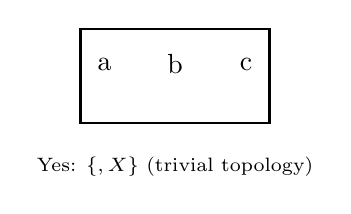
\begin{tikzpicture}[baseline=(base)]
  \node (base) at (0,0) {};
  \node at (0,0.15) {a};
  \node at (0.9,0.15) {b};
  \node at (1.8,0.15) {c};
  \draw[thick] (-0.3,-0.6) rectangle (2.1,0.6);
  \node[below=3pt] at (0.9,-0.8) {\scriptsize Yes: $\{\varnothing,X\}$ (trivial topology)};
\end{tikzpicture}
&
% 2: singletons a,b only (not a topology)
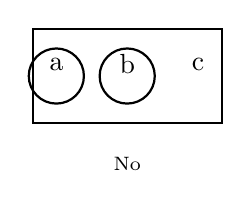
\begin{tikzpicture}[baseline=(base)]
  \node (base) at (0,0) {};
  \node at (0,0.15) {a};
  \node at (0.9,0.15) {b};
  \node at (1.8,0.15) {c};
  \draw[thick] (-0.3,-0.6) rectangle (2.1,0.6);
  \draw[thick] (0,0) circle (0.35); % {a}
  \draw[thick] (0.9,0) circle (0.35); % {b}
  \node[below=3pt] at (0.9,-0.8) {\scriptsize No};
\end{tikzpicture}
\\
% 3: two overlapping pairs (not closed under intersection -> missing {b})
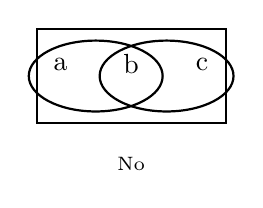
\begin{tikzpicture}[baseline=(base)]
  \node (base) at (0,0) {};
  \node at (0,0.15) {a};
  \node at (0.9,0.15) {b};
  \node at (1.8,0.15) {c};
  \draw[thick] (-0.3,-0.6) rectangle (2.1,0.6);
  \draw[thick] (0.45,0) ellipse (0.85 and 0.45); % {a,b}
  \draw[thick] (1.35,0) ellipse (0.85 and 0.45); % {b,c}
  \node[below=3pt] at (0.9,-0.8) {\scriptsize No};
\end{tikzpicture}
&
% 4: discrete with extra large circles around {a,b} and {b,c}
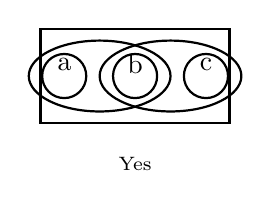
\begin{tikzpicture}[baseline=(base)]
  \node (base) at (0,0) {};
  \node at (0,0.15) {a};
  \node at (0.9,0.15) {b};
  \node at (1.8,0.15) {c};
  \draw[thick] (-0.3,-0.6) rectangle (2.1,0.6);
  % large ellipses circling {a,b} and {b,c}
  \draw[thick] (0.45,0) ellipse (0.9 and 0.45); % {a,b}
  \draw[thick] (1.35,0) ellipse (0.9 and 0.45); % {b,c}
  % individual points
  \draw[thick] (0,0) circle (0.28);
  \draw[thick] (0.9,0) circle (0.28);
  \draw[thick] (1.8,0) circle (0.28);
  \node[below=3pt] at (0.9,-0.8) {\scriptsize Yes};
\end{tikzpicture}
\\
% 5: topology with {b} and {a,b}
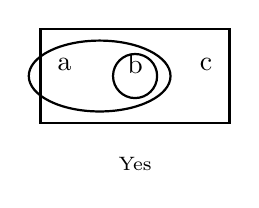
\begin{tikzpicture}[baseline=(base)]
  \node (base) at (0,0) {};
  \node at (0,0.15) {a};
  \node at (0.9,0.15) {b};
  \node at (1.8,0.15) {c};
  \draw[thick] (-0.3,-0.6) rectangle (2.1,0.6);
  \draw[thick] (0.45,0) ellipse (0.9 and 0.45); % {a,b}
  \draw[thick] (0.9,0) circle (0.28); % {b}
  \node[below=3pt] at (0.9,-0.8) {\scriptsize Yes};
\end{tikzpicture}
&
% 6: {a},{b},{a,b} present (topology)
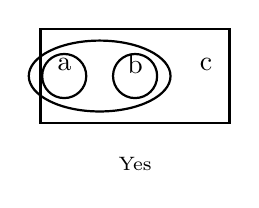
\begin{tikzpicture}[baseline=(base)]
  \node (base) at (0,0) {};
  \node at (0,0.15) {a};
  \node at (0.9,0.15) {b};
  \node at (1.8,0.15) {c};
  \draw[thick] (-0.3,-0.6) rectangle (2.1,0.6);
  \draw[thick] (0,0) circle (0.28); % {a}
  \draw[thick] (0.9,0) circle (0.28); % {b}
  \draw[thick] (0.45,0) ellipse (0.9 and 0.45); % {a,b}
  \node[below=3pt] at (0.9,-0.8) {\scriptsize Yes};
\end{tikzpicture}
\end{tikzcd}
\end{center}
\end{example}

\begin{example}
  Every metric space is a topological space with the open sets defined previously.
  
  As a special example, for $\R$, every open ball is a bounded open interval $(a,b)$. Hence, every open set in $\R$ is a union of disjoint open intervals (including unbounded intervals).

  Let $(X,\tau)$ be a topological space. If there exists a metric $d$ on $X$ such that open sets for $d$ coincide with $\tau$, we say $(X,\tau)$ is \emph{metrizable}.
\end{example}


\begin{example}
  Let $X$ be any set. Let ${\tau}:=P(X)$. Then, ${\tau}$ is a topology on $X$ and it is called the \emph{discrete topology}. This topology is induced by the discrete metric $d(x,y)=1$ if $x\neq y$ and $d(x,x)=0$.
\end{example}

\begin{example}
  Let $X$ be any set. Let ${\tau}:=\{\emptyset,X\}$. This is the \emph{trivial topology}. Is this metrizable?
\end{example}

\begin{lemma}
  For a metric space $(X,d)$, any point $x\in X$ forms a closed set, i.e., $\{x\}$ is closed.
\end{lemma}
\begin{proof}
  We show that $X\setminus\{x\}$ is open. For any $y\in X\setminus\{x\}$, let $r=d(x,y)/2>0$. Then, the open ball $B(y,r)\subseteq X\setminus\{x\}$. Hence, $X\setminus\{x\}$ is open.
\end{proof}

Now, for any set $X$ with more than two elements, the trivial topology is not metrizable since singletons are not closed.

\begin{example}
   Let $X$ be any set. Let ${\tau}:=\{O\subset X\mid O=\emptyset\ \text{or}\ X\setminus O \text{ is finite}\}$. Then ${\tau}$ is a topology on $X$ called the \emph{finite complement topology}.

    If $X=\R$, a nonempty open set is $\R$ with at most finitely many points removed. For example:
      \begin{center}
      
\begin{tikzpicture}[baseline=-1ex]
        % reduced width to fit page
        \draw[line width=6pt, green!45!black, rounded corners=1pt] (-4,0) -- (4,0);
        % small white gaps and blue open circles for removed points
        \foreach \x in {-1.5,-0.3,1.0,2.3}{
        \fill[white] (\x,0) circle (0.16); % clear the green bar
        \draw[blue, line width=0.8pt] (\x,0) circle (0.16); % open circle
        }
        % label (smaller)
        \node[below=5pt] at (0,0) {\scriptsize Nonempty open set: $\R\setminus\{x_1,\dots,x_n\}$};
      \end{tikzpicture}
      \end{center}
\end{example}
\begin{proof}
  Now we check that the finite complement topology is indeed a topology.
  \begin{itemize}
    \item The empty set and the whole space $X$ are in ${\tau}$.
    \item The intersection of finitely many open sets is open: If $U_1,\dots,U_n\in{\tau}$ then each $X\setminus U_i$ is finite. Hence
    \[
    X\setminus\bigcap_{i=1}^n U_i=\bigcup_{i=1}^n (X\setminus U_i)
    \]
    is a finite union of finite sets, hence finite. Therefore $\bigcap_{i=1}^n U_i\in{\tau}$.
    \item The union of any collection of open sets is open: If $\{U_i\}_{i\in I}\subseteq{\tau}$, then $X\setminus\bigcup_{i\in I} U_i = \bigcap_{i\in I} (X\setminus U_i)\subset X\backslash U_i$ is finite. Thus, $\bigcup_{i\in I} U_i\in{\tau}$.
  \end{itemize}
\end{proof}

The finite complement topology coincides with the trivial topology if $X$ is finite and hence is metrizable. If $X$ is infinite, the finite complement topology is not metrizable. We will need more machinery to show this.  

\begin{definition}[Comparing topologies]
Let ${\tau}$ and ${\tau}'$ be topologies on the same set $X$. If ${\tau}\subseteq{\tau}'$ we say ${\tau}$ is \emph{coarser} (or \emph{weaker}) than ${\tau}'$, and ${\tau}'$ is \emph{finer} (or \emph{stronger}) than ${\tau}$.
\end{definition}

\begin{remark}
The discrete topology $P(X)$ is the finest topology on $X$, while the trivial topology $\{\varnothing,X\}$ is the coarsest.
\end{remark}




\subsection{Basis}

Recall that in a metric space, any open set can be written as a union of open balls. So the set of open balls gives rise to a simple characterization of the metric topology. We can use this idea to define a basis for a topology.

\begin{definition}[Basis]
A \emph{basis} $\mathcal{B}$ for a topology on a set $X$ is a nonempty family of subsets of $X$ such that:
\begin{enumerate}
  \item For every $x\in X$, there exists some $B\in\mathcal{B}$ such that $x\in B$.
  \item If $x\in B_1\cap B_2$ with $B_1,B_2\in\mathcal{B}$, then there exists $B_3\in\mathcal{B}$ with $x\in B_3\subseteq B_1\cap B_2$.
\end{enumerate}
The topology generated by $\mathcal{B}$ is: any $U\subset X$ is open if for every $x\in U$, there exists $B\in\mathcal{B}$ such that $x\in B\subseteq U$. Equivalently,
\[
{\tau}_{\mathcal{B}}:=\Big\{\bigcup_{i\in I} B_i : B_i\in\mathcal{B}\Big\}.
\]
We say  “$\mathcal{B}$ is a basis for ${\tau_\mathcal{B}}$”.
\end{definition}

\begin{center}
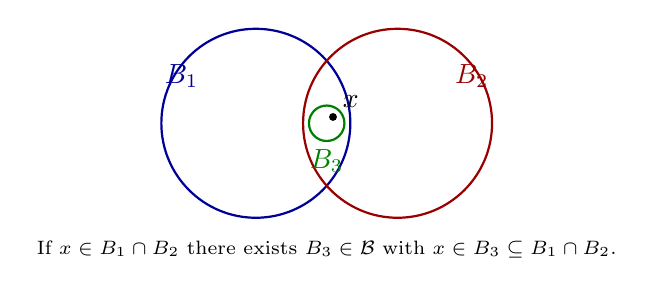
\begin{tikzpicture}[scale=1,baseline=(current bounding box.center)]
  % B1 and B2 (overlapping) - outlines only
  \draw[blue!60!black, thick] (-0.9,0) circle (1.2) node[left=6mm, yshift=6mm] {$B_1$};
  \draw[red!60!black, thick]  (0.9,0)  circle (1.2) node[right=6mm, yshift=6mm] {$B_2$};
  % B3 inside the intersection (smaller)
  \draw[green!50!black, thick] (0,0) circle (0.225) node[below=2mm] {$B_3$};
  % point x
  \filldraw[black] (0.08,0.08) circle (1.2pt) node[above right] {$x$};
  % optional intersection label
  \node at (0, -1.6) {\scriptsize If $x\in B_1\cap B_2$ there exists $B_3\in\mathcal B$ with $x\in B_3\subseteq B_1\cap B_2$.};
\end{tikzpicture}
\end{center}

\begin{example}
  Let $X$ be a metric space. Then, the collection of open balls forms a basis for the topology on $X$.
\end{example}

\begin{example}
  The collection of one point sets $\{ \{x\} : x\in X \}$ is a basis for the discrete topology on $X$.
\end{example}

\begin{example}
  Let ${\tau}$ be a topology on $X$. Then, $\mathcal{B}:={\tau}$ is a basis for ${\tau}$. This is a rather trivial case.
\end{example}

\begin{proposition}
  The topology generated by a basis is indeed a topology.
\end{proposition}
\begin{proof}
\begin{itemize}
  \item $\varnothing$ and $X$ are in ${\tau}_{\mathcal{B}}$: $\varnothing=\bigcup_{i\in\varnothing} B_i$ and $X=\bigcup_{x\in X} B_x$ where $B_x\in\mathcal{B}$ contains $x$.
  \item Arbitrary unions of sets in ${\tau}_{\mathcal{B}}$ belong to ${\tau}_{\mathcal{B}}$: Consider  $\{U_i\}_{i\in I}\subseteq{\tau}_{\mathcal{B}}$. Then, if $x\in \bigcup_{i\in I} U_i$, there exists $i_0\in I$ such that $x\in U_{i_0}$. Since $U_{i_0}$ is a union of basis elements, we can find $B\in\mathcal{B}$ with $x\in B\subseteq U_{i_0}$. Thus, $x\in B\subseteq \bigcup_{i\in I} U_i$. Hence, $\bigcup_{i\in I} U_i\in{\tau}_{\mathcal{B}}$.
  \item Now for $U_1,\ldots, U_n\in {\tau}_{\mathcal{B}}$, let $x\in U_1\cap\cdots\cap U_n$. We claim that there exists $B\in\mathcal{B}$ such that $x\in B\subseteq U_1\cap\cdots\cap U_n$. We prove by induction on $n$. The case $n=1$ is trivial. Assume the claim holds for $n=k$. Now consider $n=k+1$. By the induction hypothesis, there exists $B'\in\mathcal{B}$ such that $x\in B'\subseteq U_1\cap\cdots\cap U_k$. Since $U_{k+1}$ is open, there exists $B''\in\mathcal{B}$ such that $x\in B''\subseteq U_{k+1}$. Now, by the definition of basis, there exists $B\in\mathcal{B}$ such that $x\in B\subseteq B'\cap B''$. Hence, $x\in B\subseteq B'\cap B'' \subseteq (U_1\cap\cdots\cap U_k)\cap U_{k+1}=U_1\cap\cdots\cap U_{k+1}$. This proves the claim for $n=k+1$ and hence for all $n$.
\end{itemize}  
\end{proof}

\begin{proposition}
Let $(X,{\tau})$ be a topological space and let $\mathcal{B}\subset {\tau}$. Assume that for any $x\in U$ where $U\in {\tau}$, there exists $B\in\mathcal{B}$ with $x\in B\subseteq U$. Then $\mathcal{B}$ is a basis for ${\tau}$.
\end{proposition}
\begin{proof}
By hypothesis, for any open $U\in\tau$ and any $x\in U$ there exists $B\in\mathcal{B}$ with $x\in B\subseteq U$.

(1) Take $U=X\in\tau$. Then for every $x\in X$ there is $B\in\mathcal{B}$ with $x\in B\subseteq X$, verifying the first basis axiom.

(2) If $x\in B_1\cap B_2$ with $B_1,B_2\in\mathcal{B}\subseteq\tau$, then $U:=B_1\cap B_2\in\tau$. Applying the hypothesis to $U$ and $x$ yields $B_3\in\mathcal{B}$ such that $x\in B_3\subseteq B_1\cap B_2$, which is the second basis axiom.

Thus $\mathcal{B}$ is a basis. Let $\tau_{\mathcal{B}}$ be the topology it generates. Since $\mathcal{B}\subseteq\tau$ and $\tau$ is closed under unions, $\tau_{\mathcal{B}}\subseteq\tau$. Conversely, for any $U\in\tau$,
\[
U=\bigcup_{x\in U} B_x
\]
where each $B_x\in\mathcal{B}$ satisfies $x\in B_x\subseteq U$ by the hypothesis. Hence $U\in\tau_{\mathcal{B}}$, so $\tau\subseteq\tau_{\mathcal{B}}$. Therefore $\tau=\tau_{\mathcal{B}}$, and $\mathcal{B}$ is a basis for $\tau$.
\end{proof}

\begin{proposition}[Comparing topologies via bases]
Let $\mathcal{B}_1,\mathcal{B}_2$ be bases on $X$ generating ${\tau}_1,{\tau}_2$. Then ${\tau}_1\subseteq{\tau}_2$ iff for every $x\in X$ and $B_1\in\mathcal{B}_1$ with $x\in B_1$ there exists $B_2\in\mathcal{B}_2$ with $x\in B_2\subseteq B_1$.
\end{proposition}
\begin{proof}
($\Rightarrow$) If $B_1\in\mathcal{B}_1$, then $B_1\in{\tau}_1\subseteq{\tau}_2$ and so $B_1$ is a union of $\mathcal{B}_2$–elements. Pick one containing $x$ inside $B_1$.

($\Leftarrow$) Let $U\in{\tau}_1$; write $U=\bigcup_{i} B_i$ with $B_i\in\mathcal{B}_1$. For $x\in U$ choose $i$ with $x\in B_i$ and then $B_2\in\mathcal{B}_2$ with $x\in B_2\subseteq B_i\subseteq U$. Hence $U$ is open in ${\tau}_2$ by the basis criterion.
\end{proof}

\begin{example}
  Let $X=\R^2$. Let $\mathcal{B}=\{\text{open balls in }\R^2\}$ and let $\mathcal{B}'=\{\text{axis-aligned open rectangles in }\R^2\}$. Then they generate the same topology.
\begin{center}
  \begin{tikzcd}[column sep=12mm]
  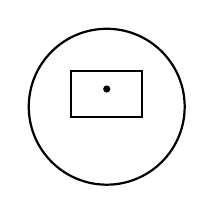
\begin{tikzpicture}[baseline=(current bounding box.center),scale=0.9]
    \draw[thick] (0,0) circle (1.1);
    \draw[thick] (-0.5,0.5) rectangle (0.5,-0.15);
    \filldraw[black] (0.0,0.25) circle (1.2pt);
  \end{tikzpicture}
  &
  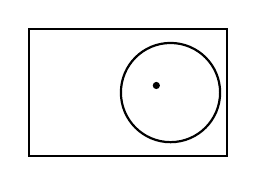
\begin{tikzpicture}[baseline=(current bounding box.center),scale=0.9]
    \draw[thick] (-1.4,-0.9) rectangle (1.4,0.9);
    \draw[thick] (0.6,0) circle (0.7);
    \filldraw[black] (0.4,0.1) circle (1.2pt);
  \end{tikzpicture}
  \end{tikzcd}
\end{center}
  
\end{example}

\subsubsection{Subbasis}

Now consider the case where we are just give a set of subsets, can we still generate a topology?

\begin{definition}[Subbasis]
A \emph{subbasis} $\mathcal{S}$ for a topology on $X$ is a collection of subsets whose union is $X$. The topology \emph{generated} by $\mathcal{S}$ is the collection of all unions of finite intersections of members of $\mathcal{S}$:
\[
{\tau}_{\mathcal{S}}=\Big\{\bigcup_{\alpha} \bigcap_{k=1}^{n_\alpha} S_{\alpha,k} : S_{\alpha,k}\in\mathcal{S},\ n_\alpha\ge 0\Big\}.
\]
\end{definition}

\begin{example}
  $\mathcal{S}=\{\{0,1\},\{0,2\}\}$ is a subbasis on $X=\{0,1,2\}$. It is clear that $\mathcal{S}$ is not a basis. The topology generated by $\mathcal{S}$ is ${\tau}_{\mathcal{S}}=\{\emptyset,\{0\},\{0,1\},\{0,2\},X\}$ with a basis $\{\{0\},\{0,1\},\{0,2\}\}$.
\end{example}

\begin{theorem}
  ${\tau}_{\mathcal{S}}$ is a topology on $X$ with the family of all finite intersections of members of $\mathcal{S}$ being a basis.
\end{theorem}
\begin{proof}
  Let $\mathcal{B}$ be the family of all finite intersections of members of $\mathcal{S}$. We first show that $\mathcal{B}$ is a basis. 

  \begin{itemize}
    \item For any $x\in X$, since $\bigcup_{S\in\mathcal{S}} S = X$, there exists $S\in\mathcal{S}$ such that $x\in S$. Hence, $x\in S\in\mathcal{B}$.
    \item For any $B_1=\bigcap_{i=1}^m S_i$ and $B_2=\bigcap_{j=1}^n S'_j$ in $\mathcal{B}$, we have that $B_1\cap B_2 = \bigcap_{i=1}^m S_i \cap \bigcap_{j=1}^n S'_j = \bigcap_{k=1}^{m+n} S_k\in \mathcal{B}$ for some $S_k\in\mathcal{S}$.
  \end{itemize}
  Then, it follows from the definition of $\tau_\mathcal{S}$ that ${\tau}_{\mathcal{S}}={\tau}_{\mathcal{B}}$.
\end{proof}

\begin{remark}
  ${\tau}_{\mathcal{S}}$ is the smallest topology containing $\mathcal{S}$, i.e., any other topology on $X$ containing $\mathcal{S}$ must also contain ${\tau}_{\mathcal{S}}$.
\end{remark}

\begin{example}
In $\R$ the open intervals $(a,b)$ form a basis. The family $\{(-\infty,a), (a,\infty): a\in\R\}$ is a subbasis generating the same topology.
\end{example}





\subsection{Kuratowski's approach}

As we've seen previously that the continuity of a function between metric spaces can be captured completely by closed sets and the notion of closure. This perspective resulted in the following definition of topology which is of course equivalent to the one given above.



\begin{definition}[Closure Operation]
Let \(X\) be a set and let
\[
\overline{\cdot} : \mathcal{P}(X) \to \mathcal{P}(X)
\]
be a map. It is called a \emph{closure operation} if for all \(A, B \subset X\):
\begin{enumerate}
  \item[(i)] \(\overline{\emptyset} = \emptyset\),
  \item[(ii)] \(A \subset \overline{A}\),
  \item[(iii)] If \(D = \overline{A}\), then \(\overline{D} = D\),
  \item[(iv)] \(\overline{A \cup B} = \overline{A} \cup \overline{B}\).
\end{enumerate}
\end{definition}

We now show that the closure operation and the topology we defined previously give rise to equivalent structures on a set. To this end, we identify the notion of a closed set in a topological space first.



\begin{proposition}
Given a topological space \((X, {\tau})\), define
\[
\overline{A} := \bigcap_{\substack{A \subset C \\ C \text{ closed}}} C.
\]
Then \(\overline{\cdot}\) is a closure operation in the sense of Definition 2.
\end{proposition}

\begin{proof}
\begin{itemize}
  \item[(i)] Since \(X\) is open, \(\emptyset\) is closed, so \(\overline{\emptyset} = \emptyset\).
  \item[(ii)] \(A\) is contained in every closed superset, so \(A \subset \overline{A}\).
  \item[(iii)] If \(D\) is closed and contains \(A\), then taking closure again yields \(D\) itself.
  \item[(iv)] For \(A,B \subset X\): $\overline{A}\cup\overline{B}$ is closed and it contains \(A \cup B\). Hence, \(\overline{A \cup B} \subseteq \overline{A} \cup \overline{B}\). Since $\overline{A}\subset \overline{A \cup B}$ and $\overline{B}\subset \overline{A \cup B}$, we conclude that \(\overline{A \cup B} = \overline{A} \cup \overline{B}\).
\end{itemize}
\end{proof}

\begin{proposition}
Conversely, if \(\overline{\cdot}\) is a closure operation as in Definition 2, then the sets
\[
\mathcal{C} := \{\overline{A} : A \subset X\}
\]
form the closed sets of a topology in the sense of Definition 1.
\end{proposition}

\begin{proof}
\begin{itemize}
  \item[(a)] From (i), \(\emptyset \in \mathcal{C}\); from (ii), \(X = \overline{X} \in \mathcal{C}\).
  \item[(b)] If \(\overline{A},\overline{B} \in \mathcal{C}\), then by (iii) and (iv), \(\overline{A} \cup \overline{B} = \overline{A \cup B} \in \mathcal{C}\). Inductively, one can show that finite unions of closed sets remain closed.
  \item[(c)] Now consider an arbitrary collection \(\{\overline{A_i}\}_{i \in I} \subseteq \mathcal{C}\). We first observe that if $A\subset B$ then $\overline{A}\subset \overline{B}$. This is due to the fact that $\overline{B}=\overline{A\cup B\setminus A}=\overline{A}\cup (B\setminus A)$. So for any $i\in I$, we have that $\overline{\bigcap_{i\in I} \overline{A_i}}\subset\overline{\overline{A}}_i=\overline{A}_i $. Therefore, \(\bigcap_{i\in I} \overline{A_i}\subseteq\overline{\bigcap_{i\in I} \overline{A_i}} \subseteq \bigcap_{i\in I} \overline{A_i}\). This implies that \(\bigcap_{i\in I} \overline{A_i} = \overline{\bigcap_{i\in I} \overline{A_i}} \in \mathcal{C}\).
\end{itemize}
\end{proof}

\subsubsection{Closure and Interior}

\begin{definition}[Interior]
Let \(X\) be a topological space and let \(A \subseteq X\). The \emph{interior} of \(A\), denoted \(\operatorname{int}(A)\) or \(\mathring{A}\), is the largest open set contained in \(A\). Equivalently, it is the union of all open sets contained in \(A\):
\[
\operatorname{int}(A) = \bigcup \{U \in \tau_X : U \subseteq A\}.
\]
\end{definition}

\begin{remark}
  For any subset $A\subset X$, we have that 
  \[
  \operatorname{int}(A) \subseteq A\subseteq \overline{A}.
  \]
\end{remark}

\begin{example}
  Let $X=\R$. Then, $\operatorname{int}((0,1]) = (0,1)$ and $\overline{(0,1]} = [0,1]$.
\end{example}

\begin{definition}
  Let $X$ be a topological space. For any $x\in X$, we say any open set containing $x$ is a \emph{(open) neighbourhood} of $x$.
\end{definition}

\begin{theorem}
  Let $X$ be a topological space and let $A\subseteq X$. Then,
  \begin{itemize}
    \item $x\in \overline{A}$ if and only if every neighbourhood of $x$ intersects $A$.
    \item $x\in \operatorname{int}(A)$ if and only if there exists a neighbourhood of $x$ contained in $A$.
  \end{itemize}
\end{theorem}

\begin{proof}
  The second item follows from the definition directly. We prove the first item below. 

  Let $x\in \overline{A}$. Assume that a neighborhood $U$ of $x$ does not intersect $A$. Then, $A\subseteq X\setminus U$. Notice that $X\backslash U$ is closed and contains $A$. Then, by definition of closure, we have $x\in \overline{A}\subseteq X\backslash U$, which is a contradiction. 

  Now, we assume $x\notin \overline{A}$. Then, there exists a closed set $C$ containing $A$ such that $x\notin C$. In particular, $x\in X\backslash C$. Note that $X\backslash C$ is open and $(X\setminus C)\cap A = \emptyset$.
\end{proof}

\newpage

\subsection{Order topology}

\begin{definition}[Linearly ordered set and intervals]
Let $(X,\le)$ be a linearly ordered (totally ordered) set. For $a,b\in X$ with $a<b$ define
\[
(a,b)=\{x\in X: a<x<b\},\quad
[a,b)=\{x\in X: a\le x<b\},
\]
\[
(a,b]=\{x\in X: a<x\le b\},\quad
[a,b]=\{x\in X: a\le x\le b\}.
\]
\end{definition}

\begin{definition}[Order topology]
Let $(X,\le)$ be a linearly ordered set with at least two elements. Let $\mathcal B$ be the family consisting of
\begin{itemize}
  \item all open intervals $(a,b)$ with $a<b$,
  \item all $[a_0,b)$ when $a_0$ is the least element of $X$ and $b>a_0$,
  \item all $(a,b_0]$ when $b_0$ is the greatest element of $X$ and $a<b_0$.
\end{itemize}
The topology generated by $\mathcal B$ is called the \emph{order topology} on $X$.
\end{definition}

\begin{proposition}
The family $\mathcal B$ above is a basis.
\end{proposition}
\begin{proof}
Nonemptiness is clear. Given $x\in X$, if $x$ is minimal, then $x$ is in $[x,b)$; if $x$ is maximal, then $x$ is in $(a,x]$; otherwise, there must exist $a,b$ such that $x\in (a,b)$. The intersection $B_1\cap B_2$ with $B_i\in\mathcal B$ must be one of the sets in $\mathcal{B}$ or emptyset.
\end{proof}

\begin{example}[Standard topology on $\R$]
With the usual order on $\R$, the sets $(a,b)$ already form $\mathcal B$, hence the order topology coincides with the usual metric topology on $\R$.
\end{example}

\begin{example}[Lexicographic order on $\R\times\R$]
Define $(x_1,y_1)<(x_2,y_2)$ iff $x_1<x_2$, or $x_1=x_2$ and $y_1<y_2$. The interval $((a,b),(c,d))$ looks like the following:


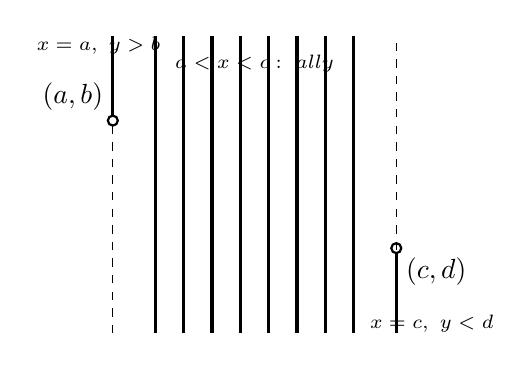
\begin{tikzpicture}[scale=0.9,baseline=(current bounding box.center)]
  % parameters
  \def\xA{0}
  \def\xC{4}
  \def\yB{1.0}
  \def\yD{-0.8}
  \def\Ymax{2.2}
  \def\Ymin{-2.0}

  % the strip a<x<c: every y is allowed (draw several full verticals)
  \foreach \x in {0.6,1.0,1.4,1.8,2.2,2.6,3.0,3.4}{
    \draw[very thick] (\x,\Ymin) -- (\x,\Ymax);
  }

  % boundary at x=a: only y>b (open at (a,b))
  \draw[very thick] (\xA,\yB) -- (\xA,\Ymax);
  \draw[fill=white,thick] (\xA,\yB) circle (2pt);
  \node[above left] at (\xA,\yB) {$(a,b)$};
  \draw[dashed] (\xA,\Ymin) -- (\xA,\Ymax);

  % boundary at x=c: only y<d (open at (c,d))
  \draw[very thick] (\xC,\Ymin) -- (\xC,\yD);
  \draw[fill=white,thick] (\xC,\yD) circle (2pt);
  \node[below right] at (\xC,\yD) {$(c,d)$};
  \draw[dashed] (\xC,\Ymin) -- (\xC,\Ymax);

  % annotations
  \node at (2.0,1.8) {\scriptsize $a<x<c:\ \text{all }y$};
  \node[above] at (-0.2,1.8) {\scriptsize $x=a,\ y>b$};
  \node[below] at (4.5,-1.6) {\scriptsize $x=c,\ y<d$};
\end{tikzpicture}

This is different from the standard topology on $\R^2$. In fact, the set above in the basis is not open in the standard topology. To see this, consider the point $(a,b+1)$ in the set. Any open ball around it will contain points with $x<a$, which are not in the set.
\end{example}

\begin{example}[Discrete order on the integers]
On $\mathbb{N}$ with the usual order, the order topology is discrete:
\[
\{n\}=(n-1,n+1)\quad\text{for }n>1;
\]
and $1$ is the least element then $\{1\}=[1,2)$. Hence every singleton is open.
\end{example}

\begin{example}[Order topology on $\{1,2\}\times\mathbb{N}$ (lexicographic) is not discrete]
Give $X=\{1,2\}\times\mathbb{N}$ the lexicographic order:
\[
(i,m)<(j,n)\quad\text{iff}\quad i<j\ \text{ or }\ (i=j\text{ and }m<n).
\]
Then $(1,1)$ is the least element. In the order topology, any basis element containing $(2,1)$ is of the form $(a,b)$ (or $[\, (1,1),b)$)
with $a<(2,1)<b$, and therefore must contain some $(1,n)$. Hence $\{(2,1)\}$ is not open, so the
order topology on $X$ is not the discrete topology.

% \begin{center}
% \begin{tikzpicture}[x=0.8cm,y=0.7cm,baseline=(current bounding box.center)]
%   % two rows of points: top is {2}xN, bottom is {1}xN
%   \foreach \k in {1,...,7}{
%     \fill (\k,0) circle (1.2pt);        % (2,k)
%     \fill (\k,-1.2) circle (1.2pt);     % (1,k)
%   }
%   % labels for a few points
%   \node[above] at (1,0) {\scriptsize $(2,1)$};
%   \node[above] at (2,0) {\scriptsize $(2,2)$};
%   \node[below] at (1,-1.2) {\scriptsize $(1,1)$};
%   \node[below] at (2,-1.2) {\scriptsize $(1,2)$};
%   \node at (7.8,-0.6) {\scriptsize $\cdots$};

%   % indicate a basic nbhd around (2,1) that must catch some (1,n)
%   \draw[thick,rounded corners,blue] (0.6,-0.35) rectangle (2.6,0.35);
%   \node[blue,above right] at (2.6,0.35) {\scriptsize neighborhood of $(2,1)$};
%   \draw[->,>=stealth,blue] (2.2,0.35) .. controls (1.9,-0.1) .. (1.6,-1.0);
%   \node[below,blue] at (1.6,-1.2) {\scriptsize some $(1,n)$};
% \end{tikzpicture}
% \end{center}
\end{example}



\subsection{Product Topology on $X\times Y$}

\begin{definition}
  Let $(X,{\tau}_X)$ and $(Y,{\tau}_Y)$ be topological spaces. The \emph{product topology} on the product space $X\times Y$ is the topology generated by the basis consisting of all products of open sets:
  \[
    \mathcal{B}_{X\times Y} = \{ U \times V : U \in {\tau}_X, V \in {\tau}_Y \}.
  \]
\end{definition}

\begin{proof}[Check: $\mathcal{B}$ is a basis]
  Note  $X\times Y\in \mathcal{B}$ so every point $(x,y)\in X\times Y$ lies in some basis element.

  For $U_1\times V_1,U_2\times V_2\in \mathcal{B}$, we have $U_1\cap U_2\in {\tau}_X$ and $V_1\cap V_2\in {\tau}_Y$, so
  \[
    (U_1\times V_1)\cap (U_2\times V_2) = (U_1\cap U_2)\times (V_1\cap V_2)\in \mathcal{B}.
  \]
\end{proof}

Question: is $\mathcal{B}$ a topology? No, the union of basis elements is not necessarily a basis element.

It turns out that smaller bases can also generate the product topology.

\begin{theorem}
  If $\mathcal{B}$ is a basis for ${\tau}_X$ and $\mathcal{B}'$ is a basis for ${\tau}_Y$, then
  \[
    \mathcal{B} \times \mathcal{B}' = \{ U \times V : U \in \mathcal{B}, V \in \mathcal{B}' \}
  \]
  is a basis for the product topology on $X \times Y$.
\end{theorem}
\begin{proof}
  Pick any $U\times V$ from the basis for the product topology. Now, for any $(x,y)\in U\times V$, we have that $x\in U$ and $y\in V$. Since $\mathcal{B}$ and $\mathcal{B}'$ are bases, there exist $U_x\in\mathcal{B}$ and $V_y\in\mathcal{B}'$ such that $x\in U_x\subseteq U$ and $y\in V_y\subseteq V$. Hence, $(x,y)\in U_x\times V_y \subseteq U\times V$. This implies that the topology generated by $\mathcal{B}\times\mathcal{B}'$ is finer than the product topology. On the other hand, since $\mathcal{B}\times\mathcal{B}'$ is a subset of the basis for the product topology, the topology generated by $\mathcal{B}\times\mathcal{B}'$ is coarser than the product topology. Therefore, they must be the same. 
\end{proof}

\begin{example}
  Let $X=Y=\R$ with the standard topology. Then, $\mathcal{B}=\{(a,b): a<b\}$ is a basis for $\R$. Hence, $\mathcal{B}\times\mathcal{B}=\{(a,b)\times(c,d): a<b, c<d\}$ is a basis for the product topology on $\R^2$. Note that $(a,b)\times(c,d)$ is an axis-aligned open rectangle in $\R^2$. Previously, we showed that this generates the same topology as the one generated by open balls in $\R^2$. So the product topology on $\R^2$ is the same as the standard metric topology on $\R^2$.
\end{example}

We can inductively define the product topology on $X_1\times X_2\times \cdots \times X_n$ for any finite $n$. But things will be a bit different for infinite products. We will discuss this later.

\begin{definition}
  Let $\pi_1:X\times Y\to X$ be defined by $\pi_1(x,y)=x$ and $\pi_2:X\times Y\to Y$ be defined by $\pi_2(x,y)=y$. The maps $\pi_1$ and $\pi_2$ are called the \emph{projections} of $X\times Y$ onto its first and second factors, respectively.
\end{definition}

Note that for any open set $U\subset X$, we have that $\pi_1^{-1}(U) = U\times Y$ and $\pi_2^{-1}(V) = X\times V$ for any open set $V\subset Y$.

\begin{theorem}
  The collection 
  \[\mathcal{S}=\{\pi_1^{-1}(U): U\in{\tau}_X\}\cup \{\pi_2^{-1}(V): V\in{\tau}_Y\}\]
  is a subbasis for the product topology on $X\times Y$.
\end{theorem}

\begin{proof}
  Note that for any $U\in\tau_X$ and $V\in\tau_Y$, we have that 
  \[U\times V = \pi_1^{-1}(U)\cap \pi_2^{-1}(V).\]
  Hence, the basis generated by $\mathcal{S}$ contains all basis elements of the product topology. On the other hand, elements in $\mathcal{S}$ are open in the product topology. Therefore, the topology generated by $\mathcal{S}$ is the same as the product topology. 
\end{proof}



\subsection{Subspace Topology}

\begin{definition}
  Suppose $(X,{\tau})$ is a topological space and let $A$ be a subset of $X$. The \emph{subspace topology} on $A$ is the collection ${\tau}_A := \{ U \cap A : U \in {\tau} \}$. Then $(A,{\tau}_A)$ is a topological space.
\end{definition}

We now check that ${\tau}_A$ is indeed a topology on $A$.
\begin{itemize}
  \item $\varnothing$ and $A$ are in ${\tau}_A$: $\varnothing = \varnothing \cap A$ and $A = X \cap A$.
  \item Arbitrary unions of sets in ${\tau}_A$ belong to ${\tau}_A$: If $\{U_i \cap A\}_{i \in I} \subseteq {\tau}_A$, then
  \[
    \bigcup_{i \in I} (U_i \cap A) = \Big(\bigcup_{i \in I} U_i\Big) \cap A \in {\tau}_A.
  \]
  \item Finite intersections of sets in ${\tau}_A$ belong to ${\tau}_A$: If $U_1 \cap A,\ldots, U_n \cap A \in {\tau}_A$, then
  \[
    (U_1 \cap A) \cap\ldots\cap (U_n \cap A) = (U_1 \cap \ldots\cap U_n) \cap A \in {\tau}_A.
  \]
\end{itemize}

\begin{example}
  $[0,1]$ is a subspace of $\mathbb{R}$. Note that $(0.5,1]$ is not open in $\R$ but open in $[0,1]$ with the subspace topology as $$(0.5,1] = (0.5,2) \cap [0,1]$$
\end{example}

\begin{lemma}
Let $(X,{\tau})$ be a topological space and $Y\subseteq X$. If $Y\in{\tau}$ and $U\in{\tau}_Y$ (i.e.\ $U$ is open in the subspace $Y$), then $U\in{\tau}$.
\end{lemma}
\begin{proof}
By definition of the subspace topology, $U\in{\tau}_Y$ means there exists $V\in{\tau}$ with $U=V\cap Y$. Since $Y\in{\tau}$ and ${\tau}$ is closed under finite intersections, $U=V\cap Y$ is open in $X$. Hence $U\in{\tau}$.
\end{proof}

\begin{lemma}
Let $(X,{\tau})$ be a topological space and let $\mathcal{B}$ be a basis for ${\tau}$. If $Y\subseteq X$ then
\[
\mathcal{B}_Y:=\{\,B\cap Y : B\in\mathcal{B}\,\}
\]
is a basis for the subspace topology ${\tau}_Y$ on $Y$.
\end{lemma}
\begin{proof}
  Given any $U\cap Y$ open ($U$ is open in $X$) in $Y$ and $y\in U\cap Y$, there exists $B\in\mathcal{B}$ such that $y\in B\subseteq U$. Then, $y\in B\cap Y\subseteq U\cap Y$. Thus, $\mathcal{B}_Y$ is a basis for $\tau_Y$.
\end{proof}

\subsubsection*{Order topology versus subspace topology}

\begin{theorem}
  If $A\subseteq X$ and $B\subseteq Y$, then the product topology on $A\times B$ is the same as the subspace topology inherited from $X\times Y$.
\end{theorem}
\begin{proof}
  Let $\mathcal{B}_X$ and $\mathcal{B}_Y$ be bases for $X$ and $Y$ respectively. Then, $\mathcal{B}_X\times \mathcal{B}_Y:=\{U\times V: U\in\mathcal{B}_X, V\in\mathcal{B}_Y\}$ is a basis for the product topology on $X\times Y$. Hence, the subspace topology of $A\times B$ has a basis
  \[\mathcal{B}_{A\times B}=\{(U\times V)\cap (A\times B): U\in\mathcal{B}_X, V\in\mathcal{B}_Y\}.\]
  Note that $(U\times V)\cap (A\times B) = (U\cap A)\times (V\cap B)$. 

  Then,
  \[
  \mathcal{B}_{A\times B}=\{(U\cap A)\times (V\cap B): U\in\mathcal{B}_X, V\in\mathcal{B}_Y\}=\mathcal{B}_A\times \mathcal{B}_B.
  \]
  This finishes the proof.
\end{proof}



\begin{theorem}
  Let $(X,d)$ be a metric space and let $Y\subseteq X$. Consider the sub metric space $(Y,d_Y)$. Then, the topology induced by $d_Y$ is the same as the subspace topology inherited from $(X,d)$.
\end{theorem}
\begin{proof}
  Let $\tau_{d_Y}$ be the topology induced by $d_Y$, and let $\tau_Y$ be the subspace topology on $Y$ inherited from the topology induced by $d$.

  Suppose first that $U\in\tau_{d_Y}$. For every $y\in U$, there exists $r>0$ such that $B_r^Y(y)\subseteq U$. Since
  \[
    B_r^Y(y)=B_r^X(y)\cap Y,
  \]
  the set $B_r^Y(y)$ is open in the subspace topology. Thus every point of $U$ has a $\tau_Y$-open neighborhood contained in $U$, so $U\in\tau_Y$.

  Conversely, suppose that $U\in\tau_Y$. Then $U=V\cap Y$ for some open set $V$ in $(X,d)$. For every $y\in U$, there exists $r>0$ such that $B_r^X(y)\subseteq V$. Hence
  \[
    B_r^Y(y)=B_r^X(y)\cap Y\subseteq V\cap Y=U.
  \]
  Therefore $U$ is open in $(Y,d_Y)$, so $U\in\tau_{d_Y}$. We conclude that $\tau_{d_Y}=\tau_Y$.
\end{proof}




Although the subspace topology and the metric topology are compatible, the order topology and the subspace topology are not always compatible. We will see when they agree.

\begin{remark}
The order and subspace topologies on a subset of a linearly ordered set need not agree.  
For instance, let \(Y=[0,1)\cup\{2\}\subset\R\) with the induced order.  
In the subspace topology, \(\{2\}\) is open in \(Y\) since \(\{2\}=(2-\tfrac12, 2+\tfrac12) \cap Y\).  
But in the order topology on \(Y\), any basis element containing \(2\) is of the form
\((a,2]_Y=\{y\in Y:a<y\le 2\}\) where $a\in Y$ (because \(2\) is the greatest element of \(Y\)),  
so it contains points of \(Y\) strictly less than \(2\); hence \(\{2\}\) is not open there.
\end{remark}

\begin{definition}[Convex subset]
Let \((X,\le)\) be a linearly ordered set. A subset \(Y\subset X\) is \emph{convex} if for all
\(a,b\in Y\) with \(a<b\) one has \((a,b)_X\subset Y\).
\end{definition}

\begin{theorem}
Let \(X\) be a linearly ordered set with the order topology, and let \(Y\subset X\) be convex (with the induced order). Then the order topology on \(Y\) coincides with the subspace topology inherited from \(X\).
\end{theorem}

For a proof, see Munkres, Theorem 16.4.
%%%%%%%%%%

\subsection{Continuous functions}

Now we consider the functions between two topological spaces.

We first define the continuity using a local idea adopted from metric spaces. Then, we will see some more global characterizations.
\begin{definition}
  A function $f:(X,{\tau}_X)\to(Y,{\tau}_Y)$ between topological spaces is called \emph{continuous} at a given point $x\in X$ if for every neighbourhood $V$ of $f(x)$ in $Y$, there exists a neighbourhood $U$ of $x$ in $X$ such that $f(U)\subseteq V$. We say that $f$ is \emph{continuous} if it is continuous at every point $x\in X$.
\end{definition}







\begin{example}
  A function $f:X\to Y$ between two metric spaces is continuous in the metric sense if and only if it is continuous in the topological sense.
\end{example}

\begin{theorem}
  Let $X$ and $Y$ be topological spaces and let $f:X\to Y$ be a function. The following are equivalent:
  \begin{enumerate}
    \item $f$ is continuous.
    \item For all open sets $H$ in $Y$, $f^{-1}(H)$ is open in $X$.
    \item For all closed sets $C$ in $Y$, $f^{-1}(C)$ is closed in $X$.
    \item For all $A\subset X$, $f(\overline{A}) \subseteq \overline{f(A)}$ (This can be thought of as the Kuratowski definition of continuity).
  \end{enumerate}
\end{theorem}

\begin{proof}

We are going to use the following observation several times:
For any $A\subseteq Y$, we have that 
\[X=f^{-1}(A)\cup f^{-1}(Y\setminus A).\]

  $(1)\Rightarrow(2)$: Let $H$ be open in $Y$. If $f^{-1}(H)=\emptyset$, then done. Otherwise, for any $x\in f^{-1}(H)$, $H$ is a neighborhood of $f(x)$. Hence, there exists a neighborhood $V$ of $x$ such that $f(V)\subseteq H$. Thus, $V\subseteq f^{-1}(H)$. Therefore, $f^{-1}(H)$ is open in $X$.

  $(2)\Rightarrow(3)$: If $C$ is closed in $Y$, then $Y\setminus C$ is open in $Y$. By (2), $f^{-1}(Y\setminus C)$ is open in $X$. Then, $f^{-1}(C)=X\setminus f^{-1}(Y\setminus C)$ is closed in $X$.

  $(3)\Rightarrow(4)$: $f^{-1}(\overline{f(A)})$ is closed by (2). Furthermore, $A\subseteq f^{-1}(\overline{f(A)})$ (since $f(A)\subseteq \overline{f(A)}$). This implies that $\overline{A} \subseteq f^{-1}(\overline{f(A)})$ and hence $f(\overline{A}) \subseteq \overline{f(A)}$.

  $(4)\Rightarrow(1)$: Let $x\in X$ and let $V$ be a neighborhood of $f(x)$ in $Y$. Set $E:=f^{-1}(Y\setminus V)=X\setminus f^{-1}(V)$. Then, we have that $f(\overline{E})\subset \overline{f(E)}\subseteq Y\setminus V$ (because $Y\setminus V$ is a closed set containing $f(E)$).

  Now we have that $x\in X\setminus \overline{E}$, which is a neighborhood of $x$. Then,
  \begin{align*}
    f(X\setminus \overline{E})\subset f(X\setminus E)=f(X\setminus f^{-1}(Y\setminus V))=f(f^{-1}(V))\subseteq V.
  \end{align*}
  This concludes the proof.
\end{proof}



\begin{remark}
  A function $f:(X,{\tau}_X)\to(Y,{\tau}_Y)$ is continuous if and only if the statement (2) holds  for all basis elements of $Y$:

  \[U=\cup B_\alpha\quad f^{-1}(U)=\cup f^{-1}(B_\alpha)\]
  \end{remark}
  
  
  \begin{remark}
  A function $f:(X,{\tau}_X)\to(Y,{\tau}_Y)$ is continuous if and only if the statement (2) holds  for all subbasis elements of $Y$:

  \[B=S_1\cap\cdots\cap S_n\quad f^{-1}(B)=\cap f^{-1}(S_i)\]
\end{remark}

\begin{remark}
  In some books, they take the (2) as the definition of continuity.
\end{remark}


\begin{example}
  Let \(f:\R\to\R\) be the constant map \(f(x)=0\). Then \(f\) is continuous, but the image of the open set \((0,1)\) is
  \[
    f((0,1))=\{0\},
  \]
  which is not open in \(\R\). Thus a continuous map need not send open sets to open sets.
\end{example}

\begin{example}
  Let $\pi:\R^2\to\R$ be the projection $\pi(x,y)=x$, which is continuous. Consider
  \[
    C=\{(x,y)\in\R^2: xy=1\},
  \]
  the hyperbola. Since $C$ is the zero set of the continuous function $f:(x,y)\mapsto xy-1$, it is closed in $\R^2$ (i.e., $C=f^{-1}(\{0\})$). But
  \[
    \pi(C)=\{x\in\R:x\neq0\}=\R\setminus\{0\},
  \]
  which is not closed in $\R$. Thus a continuous map need not send closed sets to closed sets.
\end{example}

\begin{example}
  Let $X\times Y$ be endowed with the product topology. Then, $\pi_X:X\times Y\to X$ and $\pi_Y:X\times Y\to Y$ are continuous.

  Note that for any open set $U$ in $X$, $\pi_X^{-1}(U)=U\times Y$ is open in $X\times Y$. Similarly, for any open set $V$ in $Y$, $\pi_Y^{-1}(V)=X\times V$ is open in $X\times Y$.

  Note also that the product topology $\tau_{X\times Y}$ is the smallest topology on $X\times Y$ such that both $\pi_X$ and $\pi_Y$ are continuous: any topology on $X\times Y$ that makes both $\pi_X$ and $\pi_Y$ continuous must contain a basis for $\tau_{X\times Y}$: sets of the form $U\times Y$ and $X\times V$ for all open sets $U$ in $X$ and $V$ in $Y$. 
\end{example}

\subsubsection{Constructing continuous functions}
\begin{theorem}
  \begin{enumerate}
    \item (Constant function) If $f:X\to Y$ maps all of $X$ to a single point $y_0\in Y$, then $f$ is continuous.
    \item (Inclusion) If $A$ is a subspace of $X$, the inclusion map $i:A\to X$ defined by $i(a)=a$ is continuous.
    \item (Composition) If $f:X\to Y$ and $g:Y\to Z$ are continuous, then the composition $g\circ f:X\to Z$ is continuous.
    \item (Restricting the domain) If $f:X\to Y$ is continuous and $A\subseteq X$, then the restriction $f|_A:A\to Y$ defined by $f|_A(a)=f(a)$ is continuous.
    \item (Restricting or expanding the range) Let $f:X\to Y$ be continuous. If $f(X)\subset Z\subset Y$, then the function $g:X\to Z$  obtained by restricting the range of $f$ is continuous. If $Y\subset W$, then the function $h:i_{Y\to W}\circ f:X\to W$ is continuous.
    \item (Local formulation) $f:X\to Y$ is continuous if $X=\cup U_\alpha$ for a family of open sets $U_\alpha$ and each restriction $f|_{U_\alpha}$ is continuous.
    \item (Pasting lemma) If $X=A\cup B$ with $A,B$ closed, and $f:A\to Y$, $g:B\to Y$ are continuous and agree on $A\cap B$ (i.e., $f(x)=g(x)$ for all $x\in A\cap B$), then the function $h:X\to Y$ defined by
    \[h(x)=\begin{cases}
    f(x),&x\in A\\
    g(x),&x\in B
    \end{cases}\]
    is continuous.
  \end{enumerate}
\end{theorem}

\begin{proof}
  \begin{enumerate}
    \item For any open set $U$ in $Y$, if $y_0\in U$, then $f^{-1}(U)=X$; otherwise, $f^{-1}(U)=\emptyset$. In both cases, $f^{-1}(U)$ is open in $X$. Hence, $f$ is continuous.
    \item For any open set $U$ in $X$, $i^{-1}(U)=U\cap A$ is open in $A$. Hence, $i$ is continuous.
    \item For any open set $W$ in $Z$, $(g\circ f)^{-1}(W)=f^{-1}(g^{-1}(W))$. Since $g$ is continuous, $g^{-1}(W)$ is open in $Y$. Since $f$ is continuous, $f^{-1}(g^{-1}(W))$ is open in $X$. Hence, $g\circ f$ is continuous.
    \item For any open set $U$ in $Y$, $(f|_A)^{-1}(U)=f^{-1}(U)\cap A$ is open in $A$. Hence, $f|_A$ is continuous.
    \item For any open set $V$ in $Z$, then there exists $U$ open in $Y$ such that $V=U\cap Z$. Hence, $g^{-1}(V)=f^{-1}(V)=f^{-1}(U\cap Z)$. Since $f(X)\subset Z$, we have that $f^{-1}(U\cap Z)=f^{-1}(U)$ is open in $X$. Hence, $g$ is continuous. The continuity of $h$ follows from 2 and 3.
    \item For any open set $U$ in $Y$, we first note that 
    \[f^{-1}(U)\cap U_\alpha=(f|_{U_\alpha})^{-1}(U)=\{x\in U_\alpha: f(x)\in U\}.\]
    Since $f|_{U_\alpha}$ is continuous, $(f|_{U_\alpha})^{-1}(U)$ is open in $U_\alpha$. Hence,
    \[f^{-1}(U)=\bigcup (f^{-1}(U)\cap U_\alpha)=\bigcup (f|_{U_\alpha})^{-1}(U)\] is open in $X$. This shows that $f$ is continuous.
    \item For any closed set $C$ in $Y$, $h^{-1}(C)=f^{-1}(C)\cup g^{-1}(C)$. Since $A$ and $B$ are closed, $f^{-1}(C)$ and $g^{-1}(C)$ are closed in $X$ (see the later lemma for this). Hence, $h^{-1}(C)$ is closed in $X$. This shows that $h$ is continuous.
    \begin{lemma}
  Let $A\subset X$ and let $E\subset A$. Then, $E$ is closed in $A$ if and only if there exists a closed set $F$ in $X$ such that $E=F\cap A$.
\end{lemma}
\begin{proof}
  Suppose $E$ is closed in $A$. Then $A \setminus E$ is open in $A$, so there exists an open set $U$ in $X$ such that $A \setminus E = U \cap A$. Let $F = X \setminus U$, which is closed in $X$. Then
  \[
  F \cap A = (X \setminus U) \cap A = A \setminus (U \cap A) = A \setminus (A \setminus E) = E.
  \]

  Conversely, if $E = F \cap A$ for some closed set $F$ in $X$, then
  \[
  A \setminus E = A \setminus (F \cap A) = A \cap (X \setminus F),
  \]
  where $X \setminus F$ is open in $X$. Hence, $A \setminus E$ is open in $A$, so $E$ is closed in $A$.
\end{proof}
\begin{corollary}
  Let $A\subset X$ and let $E\subset A$. If $E$ is closed in $A$ then $E$ is closed in $X$.
\end{corollary}
\begin{proof}
  Since $E$ is closed in $A$, there exists a closed set $F$ in $X$ such that $E=F\cap A$. Since $A\subset X$ is closed, we have that $E$ is closed in $X$
\end{proof}
  \end{enumerate}
\end{proof}
  


\begin{remark}
  7 is the closed set and finite version of 6. See your homework for the infinite version of 7.
\end{remark}

\begin{theorem}
  Let $f:A\to X\times Y$ be given by $f(a)=(f_X(a),f_Y(a))$. Then $f$ is continuous if and only if $f_X$ and $f_Y$ are continuous.
\end{theorem}
\begin{proof}
  Recall the projections $\pi_X:X\times Y\to X$ and $\pi_Y:X\times Y\to Y$. Note that $f_X=\pi_X\circ f$ and $f_Y=\pi_Y\circ f$. 

  $\Rightarrow$: If $f$ is continuous, then $f_X$ and $f_Y$ are continuous by the composition of continuous functions.

  $\Leftarrow$: For $U\times V$ a basis element in $X\times Y$, we have that
  \[f^{-1}(U\times V) = f^{-1}(\pi_X^{-1}(U)\cap \pi_Y^{-1}(V)) = f^{-1}(\pi_X^{-1}(U))\cap f^{-1}(\pi_Y^{-1}(V)) = f_X^{-1}(U)\cap f_Y^{-1}(V).\]
  Since $f_X$ and $f_Y$ are continuous, $f^{-1}(U\times V)$ is open in $A$. This shows that $f$ is continuous.
\end{proof}


\subsubsection{Homeomorphism}
\begin{definition}
  A function \(f: X \to Y\) between topological spaces is a \emph{homeomorphism} if it is a bijection and both \(f\) and \(f^{-1}\) are continuous. 

  If $f$ is not surjective, we let $Z=f(X)$. If the restriction $f':X\to Z$ is a homeomorphism, then we say that $f$ is a topological embedding of $X$ into $Y$.
\end{definition}

Homeomorphisms preserve topological properties, meaning that if \(X\) and \(Y\) are homeomorphic, they share all topological characteristics. More precisely, we have the following theorem.

\begin{theorem}
  Let $f:X\to Y$ be a homeomorphism. Then, $f$ induces a map $f_*:\tau_X\to\tau_Y$ defined by $f_*(U)=f(U)$ for all $U\in\tau_X$. Furthermore, $f_*$ is a bijection.
\end{theorem}
\begin{proof}
  For any $U\in\tau_X$, $f(U)=(f^{-1})^{-1}(U)$. Since $f^{-1}$ is continuous, $f(U)$ is open in $Y$. This shows that $f_*$ is well-defined.

  Next, we show that $f_*$ is injective. If $f_*(U_1)=f_*(U_2)$ for some $U_1,U_2\in\tau_X$, then $f(U_1)=f(U_2)$. Since $f$ is bijective, we have that $U_1=U_2$. This shows that $f_*$ is injective.

  Finally, we show that $f_*$ is surjective. For any $V\in\tau_Y$, since $f^{-1}$ is continuous, we have that $f^{-1}(V)$ is open in $X$. Then, 
  \[
    f_*(f^{-1}(V))=f(f^{-1}(V))=V.
  \]
  This shows that $f_*$ is surjective.

  Therefore, we conclude that $f_*:\tau_X\to\tau_Y$ is a bijection.
\end{proof}

\begin{example}
  Suppose you have a subspace in some ambient Euclidean space. You can stretch and bend it without tearing or gluing. This is a homeomorphism. For example, a coffee cup is homeomorphic to a donut (solid torus).
\end{example}

\begin{example}
  The circle and the trefoil knot are homeomorphic. But we can't deform one to the other in 3D space without cutting. 
\end{example}

\begin{example}
  The map $f:(-1,1)\to \R$ defined by $f(x)=\frac{x}{1-x^2}$ is a homeomorphism with inverse $f^{-1}: \R \to (-1,1)$ given by $f^{-1}(y)=\frac{2y}{1+\sqrt{1+4y^2}}$. So homeomorphisms need not preserve boundedness. 
\end{example}


\begin{example}[Continuous bijection not a homeomorphism]
Let
\[
X = [0, 1)
\]
with the usual topology from $\mathbb{R}$, and
\[
Y = S^1 = \{ (x,y) \in \mathbb{R}^2 : x^2 + y^2 = 1 \}
\]
with the subspace topology from $\mathbb{R}^2$.

Define
\[
f: X \to Y, \quad f(t) = (\cos 2\pi t, \sin 2\pi t).
\]
Then $f$ is a continuous bijection. However, $f^{-1}$ is not continuous: around $(1, 0) \in S^1$, neighborhoods correspond to $t$ near $0$ \emph{and} near $1$,  
  which are far apart in $[0,1)$, so $f^{-1}$ fails continuity there.

\noindent
This shows that a continuous bijection need not be a homeomorphism when the domain is not compact.
\end{example}


\begin{example}
  Is $(0,1)$ homeomorphic to $[0,1)$?
\end{example}

\begin{lemma}
  Let $f:X \to Y$ be a homeomorphism. Let $x_0\in X$. Then, the map $g:X\setminus \{x_0\} \to Y \setminus \{f(x_0)\}$ defined by $g(x) = f(x)$ is also a homeomorphism.
\end{lemma}

\begin{definition}
  Let $X$ be a topological space. We say $X$ is connected if it cannot be represented as the union of two disjoint non-empty open sets. 
\end{definition}

\begin{remark}
  If $X$ is connected and $X$ is homeomorphic to $Y$, then $Y$ is also connected. This holds obviously as the homeomorphism gives rise to a bijection between the topologies.
\end{remark}

Now we are ready to answer the previous question.

\begin{theorem}
  $(0,1)$ is not homeomorphic to $[0,1)$.
\end{theorem}
\begin{proof}
  Suppose there exists a homeomorphism $f:[0,1)\to(0,1)$. Pick any $x_0=0$ and consider the map $g:(0,1)\to(0,1)\setminus\{f(x_0)\}$ defined by $g(x)=f(x)$. By the previous lemma, $g$ is a homeomorphism. 
  Note that $(0,1)\setminus\{f(x_0)\}$ is not connected regardless the value of $f(x_0)$. However, $(0,1)=[0,1)\setminus\{x_0\}$ is connected. This is a contradiction.
\end{proof}

\begin{example}
  Similarly, we can prove that $\R$ and $\R^2$ are not homeomorphic. 
  
  How about $\R^2$ vs $\R^3$? Need algebraic topology. We will have a taste of it later in the course.
\end{example}


\subsection{Product Topology}

Recall the Cartesian product of a family of sets $\{X_i\}_{i\in I}$ is the set of functions:

\[
\prod_{i\in I} X_i := \{ x:I\to \cup_{i\in I} X_i | \text{ for all } i\in I, x(i)\in X_i \}.
\]

Let's mimic the case when $I$ is a two-point set to identify the following definition of topology.

\begin{definition}[Box topology (less important)]
For spaces $(X_i,{\tau}_i)$, $i\in I$, the \emph{box topology} on $\prod_{i\in I}X_i$ is generated by the basis
\[
\mathcal{B}_{\text{box}}=\Big\{\prod_{i\in I}U_i : U_i\in{\tau}_i\text{ for every }i\Big\}
\]
\end{definition}

Let's first verify that $\mathcal{B}_{\text{box}}$ is indeed a basis. For any $x\in \prod_{i\in I} X_i$, we have that $x\in \prod_{i\in I} X_i = \prod_{i\in I} X_i$. Furthermore, for any two basis elements $\prod_{i\in I} U_i$ and $\prod_{i\in I} V_i$, we have that
\[x\in \prod_{i\in I} (U_i\cap V_i) =\prod_{i\in I} U_i \cap \prod_{i\in I} V_i.\]
Since $U_i$ and $V_i$ are open in $X_i$, $U_i\cap V_i$ is open in $X_i$. This shows that $\mathcal{B}_{\text{box}}$ is indeed a basis.

This basis seems reasonable right? But this topology is too fine and makes many things not work. 

\begin{example}
Let $X=\R^{\N}=\prod_{n\ge1}\R$. Then, the ``diagonal'' map $f:\R\to X$ defined by $f(t)=(t,t,t,\ldots)$ is not continuous when $X$ is endowed with the box topology. Consider the open set $(-1,1)\times (-1/2,1/2)\times (-1/3,1/3)\times \cdots$. Then, 
\begin{align*}
&f^{-1}((-1,1)\times (-1/2,1/2)\times (-1/3,1/3)\times \cdots)\\
 &= f^{-1}((-1,1)\times\R\times\cdots\cap\R\times (-1/2,1/2)\times\R\times\cdots\cap\cdots)\\
&=\bigcap_{n\ge1} f^{-1}(\R\times\cdots\times (-1/n,1/n)\times \cdots)\\
&=\bigcap_{n\ge1} (-1/n,1/n) = \{0\}.
\end{align*}
Then $f^{-1}((-1,1)\times (-1/2,1/2)\times (-1/3,1/3)\times \cdots)$ is not open in $\R$. Hence, $f$ is not continuous.

\end{example}

This example actually gives us a hint how we can make things right. The problem above is that when considering the arbitrary intersection of open sets, we don't get an open set. SO, we want things to be finite in some sense. This leads to the following definition.

\begin{definition}[Product topology]
For spaces $(X_i,{\tau}_i)$, $i\in I$, the \emph{product} $X=\prod_{i\in I} X_i$ carries the product topology generated by the basis
\[
\mathcal{B}_{\text{prod}}=\Big\{\prod_{i\in I} U_i : U_i\in{\tau}_i \text{ and } U_i=X_i \text{ for all but finitely many } i\Big\}.
\]
\end{definition}

Now we verify that $\mathcal{B}_{\text{prod}}$ is indeed a basis. For any $x\in \prod_{i\in I} X_i$, we have that $x\in \prod_{i\in I} X_i = \prod_{i\in I} X_i$. Furthermore, for any two basis elements $\prod_{i\in I} U_i$ and $\prod_{i\in I} V_i$, we have that
\[\prod_{i\in I} (U_i\cap V_i) =\prod_{i\in I} U_i \cap \prod_{i\in I} V_i.\]
Since $U_i$ and $V_i$ are open in $ X_i$, $U_i\cap V_i$ is open in $X_i$. Furthermore, since $U_i=X_i$ for all but finitely many $i$ and $V_i=X_i$ for all but finitely many $i$, we have that $U_i\cap V_i=X_i$ for all but finitely many $i$. This shows that $\mathcal{B}_{\text{prod}}$ is indeed a basis.

\begin{remark}
  Since $\mathcal{B}_{\text{prod}} \subseteq \mathcal{B}_{\text{box}}$, the product topology is coarser than the box topology. If the index set $I$ is finite, then the box topology and the product topology coincide.
\end{remark}



\begin{remark}
  The identity map $(\prod_{i\in I} X_i,{\tau}_{\text{box}})\to(\prod_{i\in I} X_i,{\tau}_{\text{prod}})$ is continuous; the inverse need not be when $I$ is infinite.
\end{remark}

\begin{example}
Now we revisit this example where $X=\R^{\N}=\prod_{n\ge1}\R$. Then, the ``diagonal'' map $f:\R\to X$ defined by $f(t)=(t,t,t,\ldots)$ is continuous when $X$ is endowed with the product topology. Consider any basis element $U=\prod_{n\ge1} U_n$ in $X$. Then, there exists $N>0$ such that for all $n>N$, $U_n=\R$. Then,
\begin{align*}
&f^{-1}(\prod_{n\ge1} U_n) = f^{-1}(\prod_{n=1}^N U_n \times \prod_{n>N} \R)\\
&=f^{-1}(\bigcap_{n=1}^N \R\times\cdots\times U_n\times \R\times\cdots) \\
&= \bigcap_{n=1}^N f^{-1}(\R\times\cdots\times U_n\times \R\times\cdots)\\
&=\bigcap_{n=1}^N U_n.
\end{align*}
Since $(U_n)$ is open in $\R$ for all $n$, $f^{-1}(\prod_{n\ge1} U_n)$ is open in $\R$. Hence, $f$ is continuous.

\end{example}




\begin{example}
Let $X=\R^{\N}=\prod_{n\ge1}\R$. Then $(0,1)^\N$ is box open but not product open (it contains no basis element). 
\end{example}

The product topology has a simple subbasis.

\begin{theorem}
  The product topology on $X=\prod_{i\in I}X_i$ is generated by the subbasis
  \[
  \mathcal{S}=\{\pi_i^{-1}(U_i): i\in I, U_i\text{ open in } X_i\}
  \]
  where $\pi_i:X\to X_i$ is the projection onto the $i$th factor.
\end{theorem}
\begin{proof}
  Note that for any $i\in I$ and any open set $U_i$ in $X_i$, $\pi_i^{-1}(U_i)$ is of the form
  \[\pi_i^{-1}(U_i) = \prod_{j\in I} V_j\]
  where $V_j = U_i$ if $j=i$ and $V_j = X_j$ otherwise.

  So, for any finite family of such sets $\pi_{i_1}^{-1}(U_{i_1}),\ldots,\pi_{i_n}^{-1}(U_{i_n})$, we have that
  \[\bigcap_{k=1}^n \pi_{i_k}^{-1}(U_{i_k}) = \prod_{j\in I} W_j\]
  where $W_j = U_{i_k}$ if $j=i_k$ for some $k\in\{1,\ldots,n\}$ and $W_j = X_j$ otherwise. This is a basis element in the product topology.

  Conversely, it is easy to see that any basis element $\prod_{i\in I} U_i$ in the product topology can be written as a finite intersection of sets in $\mathcal{S}$ as above.
\end{proof}


Here is a one great example showing why people care about the product topology.

\begin{definition}
  Let $\pi_i:\prod_{j\in I} X_j\to X_i$ be the projection onto the $i$th factor, i.e., $\pi_i(x) = x(i)$. 
\end{definition}

\begin{theorem}[Minimality]
Let ${\tau}_{\Pi}$ be the product topology on $X=\prod_{i\in I}X_i$. It is the smallest topology on $X$ making every projection $\pi_i:X\to X_i$ continuous: if ${\tau}$ is any topology on $X$ with all $\pi_i$ continuous, then ${\tau}_{\Pi}\subseteq {\tau}$.
\end{theorem}

\begin{proof}
  For any $U_i$ open in $X_i$, we have that $\pi_i^{-1}(U_i)$ must be contained in $\tau$. So $\tau\supset \mathcal{S}$ and hence $\tau\supset \tau_\Pi$.
\end{proof}

\begin{theorem}\label{theorem: product continuous}
  Consider any function $f:Y\to \prod_{j\in I} X_j$. Then $f$ is continuous iff each coordinate projection $f_i:=\pi_i\circ f:Y\to X_i$ is continuous.
\end{theorem}
\begin{proof}
  Note each projection $\pi_i$ is continuous by the theorem above.

  $\Rightarrow$: If $f$ is continuous, then $f_i=\pi_i\circ f$ is continuous by the composition of continuous functions.

  $\Leftarrow$: For any subbasis element $\pi_{i}^{-1}(U_{i})$ where $U_i$ is open in $X_i$, we have that $f^{-1}(\pi_{i}^{-1}(U_{i})) = (\pi_i \circ f)^{-1}(U_i) = f_i^{-1}(U_i)$ is open in $Y$ since $f_i$ is continuous. This proves that $f$ is continuous.
\end{proof}

\begin{remark}
  The $\Leftarrow$ direction needs not be true if we consider the box topology instead of the product topology. The same diagonal map $f:\R\to\R^\N$ defined by $f(t)=(t,t,t,\ldots)$ is a counterexample: every $f_i(t)=t$ is continuous but $f$ is not continuous when $\R^\N$ is endowed with the box topology.
\end{remark}


Now let's talk about the product of metric spaces. We have one example in homework 3  but we will give a more general construction here.

\begin{lemma}
  Let $(X,d)$ be a metric space. Define $d':X\times X\to\R$ by
  \[d'(x,y)=\min\{d(x,y),1\}.\]
Then, $d'$ is a metric on $X$ and the topology induced by $d'$ is the same as the topology induced by $d$.
\end{lemma}
\begin{proof}
  It is easy to check that $d'$ is a metric. 

  Since $d'(x,y)\le d(x,y)$, then $\tau_{d'}\subset \tau_d$.

  Now, we show that $\tau_d\subset \tau_{d'}$. For any $x\in X$ and any $r>0$, if $r\le 1$, then $B_d(x,r)=B_{d'}(x,r)$; if $r>1$, then $B_d(x,r)\supset B_{d'}(x,1)$. This shows that $\tau_d\subset \tau_{d'}$.
\end{proof}
\begin{theorem}
  Let $\{(X_i,d_i)\}_{i\in\N}$ be a family of metric spaces. Let $X=\prod_{i\in \N} X_i$. For any $i\in \N$, we define $d_i':X\times X\to\R$ by
  \[d_i'(x,y)=\min\{d_i(x(i),y(i)),1\}.\]
Then, the function $d:X\times X\to\R$ defined by
\[d(x,y)=\sum_{i\in \N} \frac{d_i'(x,y)}{2^i}\]
is a metric on $X$ and the topology induced by $d$ is the product topology.
\end{theorem}

The proof is going to be almost identical to problem 3 in homework 3. So we omit it here.


\begin{example}
  $\R^\N$ with the box topology is not metrizable. Let $A=\{(x_1,\ldots)|x_i>0\}$ and let $\mathbf{0}=(0,0,\ldots)$. Then, $\mathbf{0}\in \overline{A}$: for any basis element $U=(a_1,b_1)\times (a_2,b_2)\times\cdots$ containing $\mathbf{0}$, we have that $a_i<0<b_i$ for all $i$. So pick any point $(x_1,x_2,\ldots)$ with $x_i\in (0,b_i)$ for all $i$, then $(x_1,x_2,\ldots)\in A\cap U$. So, $\overline{A}\cap U\neq\emptyset$.

Assume that $\R^\N$ with the box topology is metrizable with a compatible metric $d$. Let $\mathbf{a}_n=(x_{1n},x_{2n},\ldots)$ be a sequence in $A$ converging to $\mathbf{0}$. Then, construct $B=\{(-x_{11},x_{11})\times (-x_{22},x_{22})\times \cdots\}$. Then, $\mathbf{0}\in B$ but $\mathbf{a}_n\notin B$ for all $n\in\N$. So there exists a ball $B_r(\mathbf{0})\subseteq B$ for some $r>0$ containing no point in the sequence $\mathbf{a}_n$. This is a contradiction. So $\R^\N$ with the box topology is not metrizable.

\end{example}


\newpage

\subsection{Quotient spaces}

We have seen how to construct topologies on various sets. One way to create a new space from old ones is via gluing. More precisely, let $X$ be a topological space and let $X^*$ be a partition of $X$ (in other words, an equivalence relation $\sim$ on $X$ so that $X^*=X/\sim$).


\begin{example}
  One can obtain a torus and a sphere via gluing/equivalence relations.
\begin{figure}[h!]
\centering
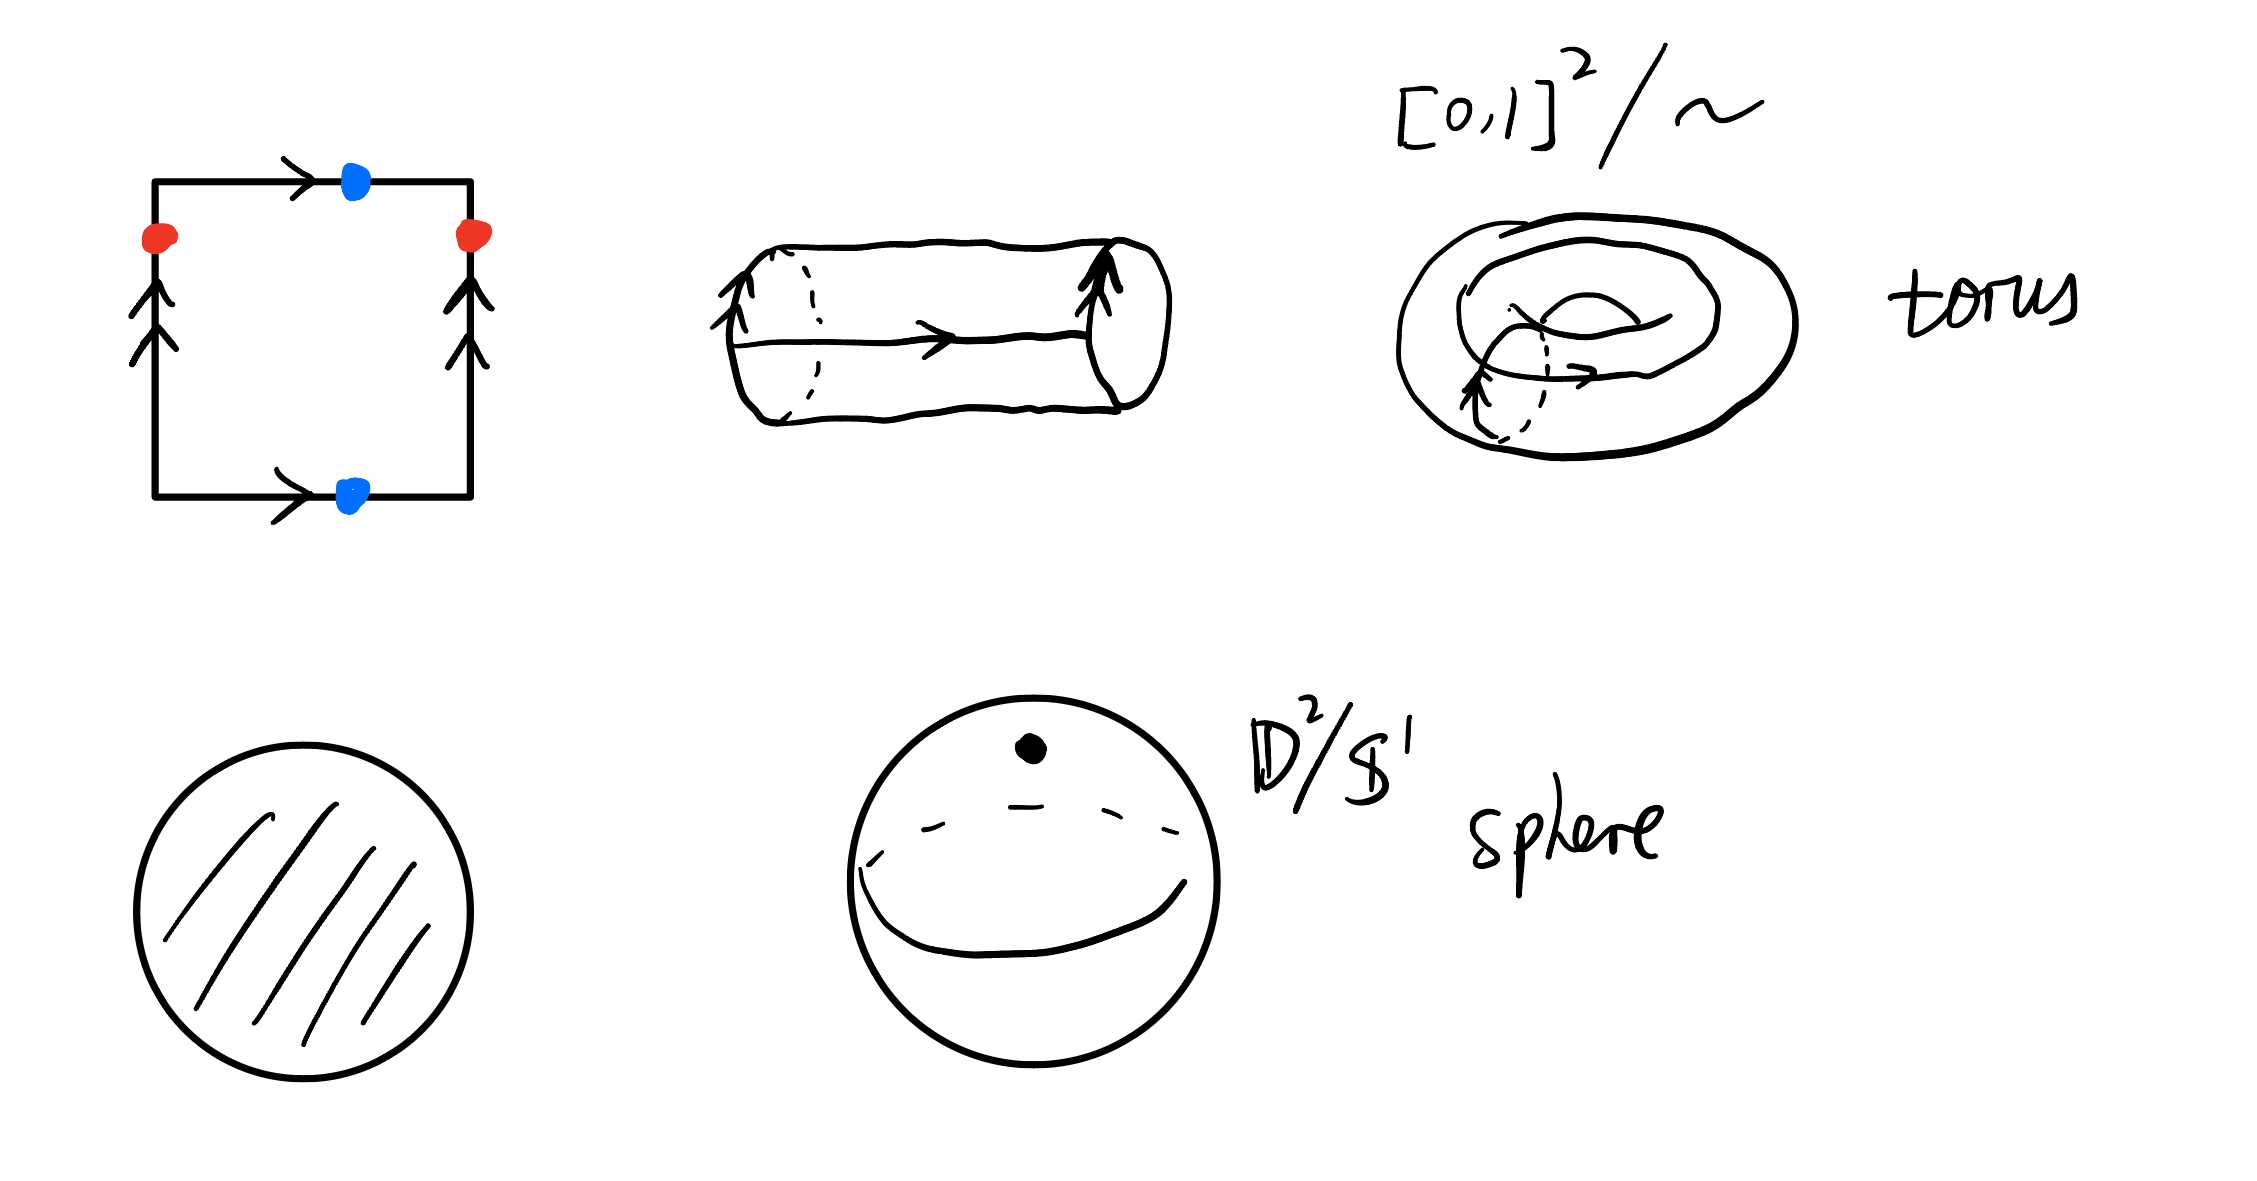
\includegraphics[width=0.8\textwidth]{figures/torus-sphere.png}
\caption{A torus and a sphere, illustrating the concept of quotient spaces.}
\label{fig:torus-sphere}
\end{figure}

\end{example}

How can we get a topology on $X^*$ from the topology on $X$? Recall that the product topology can be characterized via some continuous maps. Maybe we can do something similar here. A very natural map is the quotient map $p:X\to X^*$ sending each point to its equivalence class.

We want the finest topology on $X^*$ that makes $p$ continuous. Thus we declare a subset $U\subseteq X^*$ to be open whenever $p^{-1}(U)$ is open in $X$. This includes every subset that can be open without violating continuity of $p$.




% The product topology on $X=\Pi X_i$ is the weakest topology so that all projections $\pi_i:X\to X_i$ are continuous. Dually, we may consider the strongest topology on $Y$ so that maps $q_i:X_i\to Y$ are continuous. If we just consider one surjective map, we obtain the notion of quotient topology.


\begin{definition}[Quotient topology]
Let $q:X\to Y$ be a surjective map. The \emph{quotient topology} on $Y$ is defined by
\[\tau_q: = \{ V \subseteq Y \mid q^{-1}(V) \text{ is open in } X \}\]
When endowed with the quotient topology, we call $Y$ a \emph{quotient space} of $X$ and $q$ a \emph{quotient map}.
\end{definition}
\begin{proof}[Check: this is indeed a topology]
  $q^{-1}(Y)=X$ and $q^{-1}(\emptyset)=\emptyset$. So $Y,\emptyset\in\tau_q$.

  $q^{-1}(\bigcup_{\alpha} V_\alpha) = \bigcup_{\alpha} q^{-1}(V_\alpha)$, so $\bigcup_{\alpha} V_\alpha \in \tau_q$.

  $q^{-1}(\cap_{i=1}^nV_i) = \cap_{i=1}^n q^{-1}(V_i)$, so $\cap_{i=1}^n V_i \in \tau_q$. 
\end{proof}

\begin{remark}
  The quotient topology is the finest topology on $Y$ making $q$ continuous: if $\tau$ is any topology on $Y$ with $q$ continuous, then $\tau\subseteq \tau_q$.
\end{remark}

\begin{definition}[Quotient space]
  Let $X$ be a topological space. Let $\sim$ be an equivalence relation on $X$ and let $X^*:=X/\sim$ be the set of equivalence classes. The \emph{quotient space} of $X$ by $\sim$ is the set $X^*$ endowed with the quotient topology via the natural projection map $p:X\to X^*$ sending each point to its equivalence class.
\end{definition}

% \begin{remark}
%   Note that we start with $q:X\to X^*$ and then turn to a general surjective map $q:X\to Y$. You should think of $Y$ as $X^*$. Indeed, any surjective map $q:X\to Y$ induces an equivalence relation $\sim$ on $X$ defined by $x\sim x'$ iff $q(x)=q(x')$. Then, $Y$ is in bijection with $X^*=X/\sim$ via the map sending each equivalence class to its image under $q$. So we can identify $Y$ with $X^*$.
%   \begin{center}
%   \begin{tikzcd}[column sep=large]
%   X \arrow[drr, two heads, "q"'] \arrow[rr, two heads, "p"] && X/{\sim} \arrow[d,"\varphi","\cong"'] \\
%   && Y
%   \end{tikzcd}
%   \end{center}

%   More explicitly, let $p:X\to X^*$ be the natural projection. Then we have the quotient topology on $X^*$: 
%   \[\tau_p=\{V\subseteq X^*: p^{-1}(V)=\{x|[x]\in V\} \text{ is open in } X\}.\]

  

% \end{remark}

\begin{example}[A 3–point quotient of $\R$]
Let $p:\R\to Y=\{-1,0,1\}$ be
\[
p(x)=
\begin{cases}
-1,&x<0,\\
0,&x=0,\\
1,&x>0.
\end{cases}
\]
Endow $Y$ with the quotient topology via $p$. A subset $V\subseteq Y$ is open iff $p^{-1}(V)$ is open in $\R$.

\begin{itemize}
  \item $p^{-1}(\{-1\})=(-\infty,0)$ and $p^{-1}(\{1\})=(0,\infty)$ are open $\Rightarrow \{-1\},\{1\}$ are open.
  \item $p^{-1}(\{0\})=\{0\}$ is not open $\Rightarrow \{0\}$ not open.
  \item $p^{-1}(\{-1,1\})=\R\setminus\{0\}=(-\infty,0)\cup(0,\infty)$ is open $\Rightarrow \{-1,1\}$ open.
  \item $p^{-1}(\{-1,0\})=(-\infty,0]$ and $p^{-1}(\{0,1\})=[0,\infty)$ are not open.
\end{itemize}

Thus
\[
\tau_Y=\{\varnothing,\{-1\},\{1\},\{-1,1\},\{-1,0,1\}\}.
\]
\end{example}

\begin{figure}[htbp!]
  \centering
  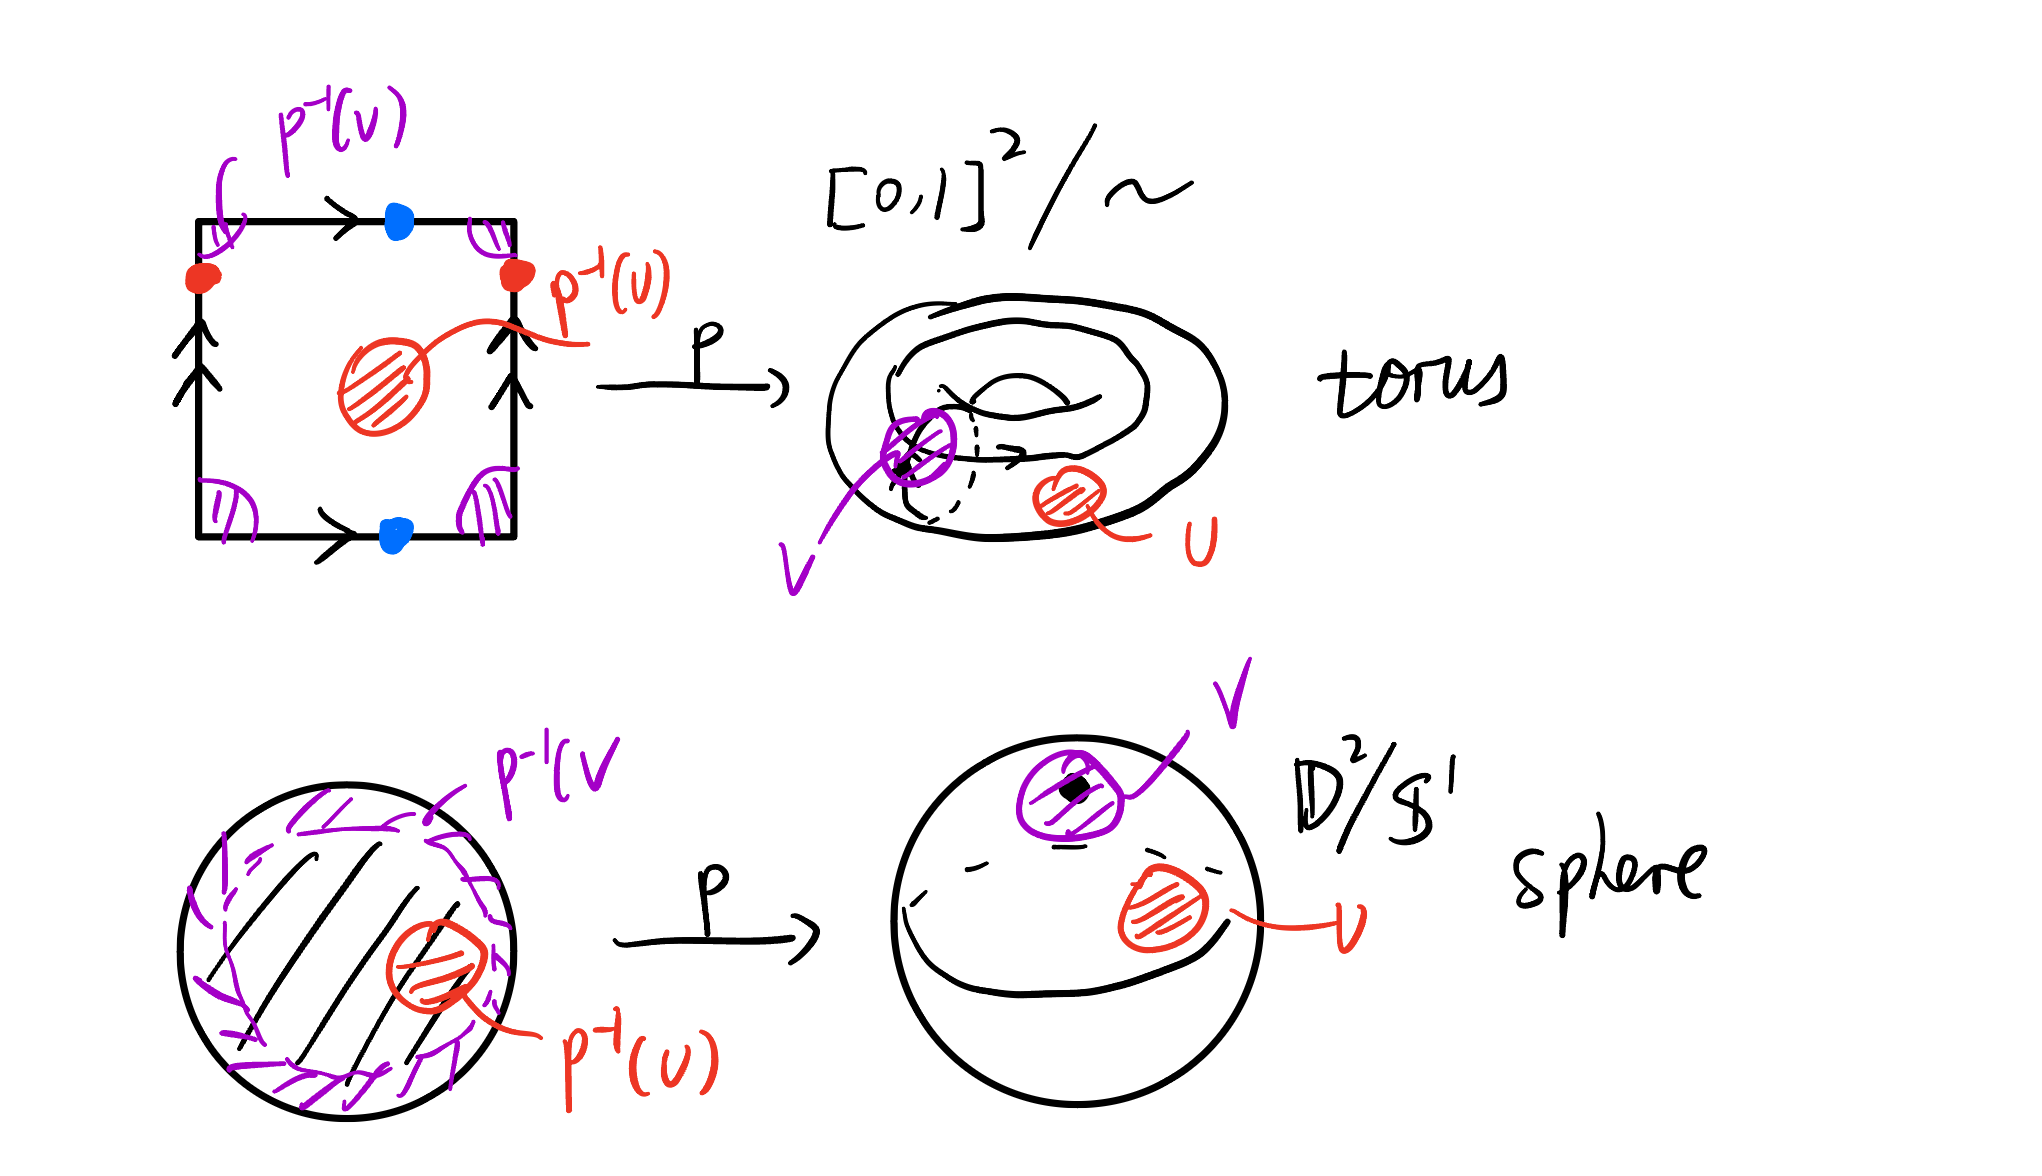
\includegraphics[width=0.8\textwidth]{figures/torus-sphere-subspace.png}
  \caption{A torus and a sphere, illustrating the concept of quotient spaces.}
  \label{fig:torus-sphere-subspace}
  \end{figure}

\begin{example}[Torus and Sphere]
  Consider the maps shown in the image (Figure \ref{fig:torus-sphere-subspace}). We then can endow the torus and the sphere (viewed as subsets of $\R^3$) with the quotient topologies via these maps. Of course, there is the question whether these quotient topologies coincide with the subspace topologies from $\R^3$. We will answer this question later.
\end{example}



\newpage

Now let $q:X\to Y$ be surjective. What if we have another topology $\tau$ on $Y$?

\begin{definition}
  For two topological spaces $X,Y$ and a surjective map $q:X\to Y$, we say $q$ is a \emph{quotient map} if 

  \[\text{a subset $U \subseteq Y$ is open in $Y$ iff $q^{-1}(U)$ is open in $X$.}\]
\end{definition}

In other words, $q$ is a quotient map if the topology on $Y$ coincides with the quotient topology via $q$. 

Whenever we have a quotient map $q:X\to Y$, we can identify $Y$ with the quotient space $X^*$ of $X$ by the equivalence relation induced by $q$. More precisely, we have the following proposition.

\begin{proposition}
  Let $q:X\to Y$ be a quotient map. Define $\sim$ on $X$ by $x\sim x'$ iff $q(x)=q(x')$ and let $X^*:=X/\sim=\{q^{-1}(y): y \in Y\}$ endowed with the quotient topology. Then, $q$ induces a homeomorphism $\varphi:X^*\to Y$ such that the following diagram commutes:
  \begin{center}
  \begin{tikzcd}[column sep=large]
  X \arrow[drr, two heads, "q"'] \arrow[rr, two heads, "p"] && X^{*} \arrow[d,"\varphi"] \\
  && Y
  \end{tikzcd}
  \end{center}
\end{proposition}
\begin{proof}
  We first define $\varphi:X^*\to Y$ by $\varphi(q^{-1}(y))=y$. This is well-defined since $q^{-1}(y)=q^{-1}(y')$ implies $y=y'$. It is easy to see that $\varphi$ is bijective and the diagram commutes.

  Next, we show that $\varphi$ is continuous. For any open set $U\subseteq Y$, we have that
  \[p^{-1}(\varphi^{-1}(U))=q^{-1}(U)\]
is open since $q$ is continuous. By the definition of the quotient topology, $\varphi^{-1}(U)$ is open in $X^*$ and hence $\varphi$ is continuous.

Finally, we show that $\varphi^{-1}$ is continuous. For any open set $V\subseteq X^*$, we have that
\[q^{-1}(\varphi(V))=p^{-1}(V)\]
is open since $p$ is continuous. By the definition of the quotient map, $\varphi(V)$ is open in $Y$ and hence $\varphi^{-1}$ is continuous.
\end{proof}


Here is some simple criterion for quotient maps. A map is said to be \emph{open} if the image of every open set is open. Similarly, a map is said to be \emph{closed} if the image of every closed set is closed.

\begin{theorem}
  Let $q:X\to Y$ be a surjective continuous map. If $q$ is open or closed, then $q$ is a quotient map.
\end{theorem}
\begin{proof}
  We only need to show the ``only if'' direction. Suppose $q$ is open. Let $U\subseteq Y$ be such that $q^{-1}(U)$ (we used surjection here) is open in $X$. Then, $U=q(q^{-1}(U))$ is open in $Y$ since $q$ is open.   
  The case when $q$ is closed is similar.
\end{proof}



\begin{example}[A quotient map that is neither open nor closed]
  Let $A=[0,1)\subset\R$. Identify all points of $A$ with one another and leave every other point distinct: define $x\sim y$ if $x=y$ or both $x,y\in A$. Give $Y=\R/{\sim}$ the quotient topology and let $q:\R\to Y$ be the natural projection. Then $q$ is a quotient map.

  Write $*$ for the point corresponding to $A$. Since
  \[
    q^{-1}(\{*\})=[0,1)
  \]
  is neither open nor closed in $\R$, the singleton $\{*\}$ is neither open nor closed in $Y$.
  But $q((0,1))=\{*\}$ although $(0,1)$ is open, and $q(\{0\})=\{*\}$ although $\{0\}$ is closed. Thus $q$ is neither an open map nor a closed map, so the converse of the preceding theorem fails.
\end{example}

\begin{example}
  Consider the subspace
  \[
  X=\{(x,y)\in\R^2: xy=1\}\ \cup\ \{(0,0)\}\subset\R^2,
  \qquad
  q:X\longrightarrow \R,\; q(x,y)=x.
  \]
  The map \(q\) is surjective: for \(x\neq 0\) choose \(y=1/x\), and \(q(0,0)=0\).
  It is continuous as the restriction of the projection \(\pi_1:\R^2\to\R\).

  However \(q\) is not a quotient map.
  Indeed \(\{(0,0)\}=B_\varepsilon(0,0)\cap X\) for small \(\varepsilon>0\), so \(\{(0,0)\}\) is open in \(X\).
  Thus
  \[
  q^{-1}(\{0\})=\{(0,0)\}\ \text{ is open in } X,
  \]
  but \(\{0\}\) is not open in \(\R\). Thus \(q\) is continuous and surjective, but not a quotient map.
\end{example}

\begin{example}
  Let $X=[0,2\pi]$ with the usual topology from $\R$. Let $Y=S^1=\{(x,y)\in\R^2:x^2+y^2=1\}$ with the subspace topology from $\R^2$. Define
  \[
  p:X\to Y,\quad p(t)=(\cos t,\sin t).
  \]
  Then, $p$ is surjective and continuous. $p$ is not open unfortunately: $[0,a)$ will not be mapped to an open set. But $p$ is closed. Later when we have more tools, this can be proved easily. But now, let's use techniques we have to prove it.

  \begin{proof}[Proof that $p$ is closed]
  Let $F\subset[0,2\pi]$ be closed. We show $p(F)$ is closed in $S^{1}$.
  Since $S^{1}\subset\R^{2}$ is a metric space, it suffices to use sequences.

  Take any sequence $(y_n)\subset p(F)$ with $y_n\to y\in S^{1}$. For each $n$ choose
  $t_n\in F$ such that $p(t_n)=y_n$. The sequence $(t_n)$ lies in the bounded interval
  $[0,2\pi]$, so by Bolzano–Weierstrass it has a convergent subsequence
  $t_{n_k}\to t\in[0,2\pi]$. Because $F$ is closed and each $t_{n_k}\in F$, we have $t\in F$.
  By continuity of $p$,
  \[
  p(t_{n_k}) \longrightarrow p(t).
  \]
  But $p(t_{n_k})=y_{n_k}\to y$, hence $y=p(t)\in p(F)$. Thus every limit of a convergent
  sequence in $p(F)$ lies in $p(F)$; so $p(F)$ is closed in $S^{1}$.

  Therefore $p$ sends closed subsets of $[0,2\pi]$ to closed subsets of $S^{1}$, i.e.\ $p$ is a
  closed map. Since $p$ is surjective and continuous, it is a quotient map.
  \end{proof}

  In this way, we can identify $S^1$ with the quotient space obtained by attaching end points of an interval $[0,2\pi]/(0\sim 2\pi)$.
\end{example}

\begin{remark}
  The gluing maps in the interval, torus, and sphere examples above are quotient maps when the targets are endowed with subspace topologies. In fact, these maps are closed, which we can prove later when we learn about compactness. Right now, we can just use the sequence argument as in the previous example.
\end{remark}



\subsubsection{Universal properties: products and quotients}

Both constructions can be described by how continuous maps factor through them. For a product, we specify a map \emph{into} the product by its coordinates. For a quotient, we obtain a map \emph{out of} the quotient from a map that is constant on each fiber. In each case, the resulting map is unique.

Here \emph{universal} means that the property holds for every topological space $Z$ and every choice of maps satisfying the stated conditions.

\begin{theorem}[Universal property of the product]
\label{theorem: product universal property}
Let $\{X_i\}_{i\in I}$ be a family of topological spaces, and let $P=\prod_{i\in I}X_i$ have the product topology, with coordinate projections $\pi_i:P\to X_i$. Let $Z$ be any topological space and let $g_i:Z\to X_i$ be a function for each $i\in I$. Then there is a unique function $g:Z\to P$ such that
\[
  \pi_i\circ g=g_i\qquad\text{for every }i\in I.
\]
It is defined by $g(z)=(g_i(z))_{i\in I}$. Moreover, $g$ is continuous if and only if $g_i$ is continuous for every $i\in I$.
\end{theorem}

The following diagram commutes for every $i\in I$:
\begin{center}
\begin{tikzcd}[column sep=3.2em,row sep=3.2em]
Z \arrow[r,dashed,"g"] \arrow[dr,"g_i"'] & P \arrow[d,"\pi_i"] \\
& X_i
\end{tikzcd}
\end{center}
\begin{proof}
The formula $g(z)=(g_i(z))_{i\in I}$ defines a function $g:Z\to P$ with $\pi_i\circ g=g_i$ for every $i\in I$. If $h:Z\to P$ also satisfies these identities, then $h(z)$ and $g(z)$ have the same coordinates for every $z\in Z$. Hence $h=g$.

If $g$ is continuous, then each $g_i=\pi_i\circ g$ is continuous, since the projections are continuous. Conversely, if every $g_i$ is continuous, then $g$ is continuous by Theorem~\ref{theorem: product continuous}.
\end{proof}

\begin{theorem}[Universal property of a quotient map]
Let $q:X\to Y$ be a quotient map and let $Z$ be a topological space. Let $g:X\to Z$ be such that $g$ is constant on each fiber $q^{-1}(\{y\})$. Then there is a unique function $f:Y\to Z$ such that $f\circ q=g$, defined by $f(q(x))=g(x)$. Moreover,
\begin{enumerate}
  \item $f$ is continuous iff $g$ is continuous.
  \item $f$ is a quotient map iff $g$ is a quotient map.
\end{enumerate} 
\end{theorem}

\begin{center}
\begin{tikzcd}[column sep=3.2em,row sep=3.2em]
X \arrow[d,"q"'] \arrow[dr,"g"] & \\
Y \arrow[r,dashed,"f"'] & Z
\end{tikzcd}
\end{center}

% \begin{theorem}
% Let $q:X\to Y$ be a quotient map and let $Z$ be a topological space. Let $g:X\to Z$ be \emph{constant on each }  $q^{-1}(\{y\})$. This induces a function $f:Y\to Z$ such that $f\circ q=g$. Then  $f$ is continuous iff $g$ is continuous. 
% \end{theorem}

\begin{proof}
The formula $f(q(x))=g(x)$ is well-defined because $g$ is constant on each fiber of $q$. Since $q$ is surjective, this formula defines $f$ on all of $Y$ and determines it uniquely.

(1) $(\Rightarrow)$ Composition of continuous maps is continuous.

$(\Leftarrow)$ Suppose $g$ is continuous. Let $V\subseteq Z$ be open. Then
\[
(f\circ q)^{-1}(V)=q^{-1}\bigl(f^{-1}(V)\bigr)
\]
is open in $X$. Since $q$ is a quotient map, $f^{-1}(V)$ is open in $Y$; hence $f$ is continuous.


(2) Since $q$ is surjective, $f$ is surjective if and only if $g$ is; their continuity is equivalent by (1). It remains to check the condition on open sets.

$(\Leftarrow)$ Suppose $g$ is a quotient map. Let $U\subseteq Z$ be such that $f^{-1}(U)$ is open in $Y$. Then
\[q^{-1}(f^{-1}(U))=(f\circ q)^{-1}(U)=g^{-1}(U)\]
is open in $X$. Since $g$ is a quotient map, $U$ is open in $Z$. Hence $f$ is a quotient map.

$(\Rightarrow)$ Suppose $f$ is a quotient map. Let $U\subseteq Z$ be such that $g^{-1}(U)$ is open in $X$. Then
\[q^{-1}(f^{-1}(U))=(f\circ q)^{-1}(U)=g^{-1}(U)\]
is open in $X$. Since $q$ is a quotient map, $f^{-1}(U)$ is open in $Y$. Since $f$ is a quotient map, $U$ is open in $Z$. Hence $g$ is a quotient map. The same proof shows that the composition of two quotient maps is a quotient map.
\end{proof}

% As a consequence, we prove the other direction of a quotient map proposition above.

% \begin{corollary}
%   Let $q:X\to Y$ be a surjective continuous map and let $X^*=\{q^{-1}(\{y\}): y \in Y\}$ endowed with the quotient topology. 
%   Then, the map $q$ induces a bijective continuous map $\varphi:X^*\to Y$, which is a homeomorphism iff $q$ is a quotient map.
% \end{corollary}

% \begin{proof}


%   We already proved the if part.

%   For the only if part, 
%   It is easy to see that $\varphi$ is bijective. If $\varphi$ is a homeomorphism, then $\varphi^{-1}$ is continuous. By the theorem above, $p\circ \varphi^{-1}$ is continuous iff $\varphi^{-1}$ is continuous. But $p\circ \varphi^{-1}=q$. So $q$ is a quotient map.
% \end{proof}



% \begin{example}[Circle as a quotient]
% Identify $0\sim 1$ in $[0,1]$; let $p:[0,1]\to [0,1]/(0\sim 1)$. Define
% \[
% g:[0,1]\to S^{1},\qquad g(t)=(\cos 2\pi t,\sin 2\pi t).
% \]
% Then $g(0)=g(1)$, so $g$ is constant on fibers of $p$. By the theorem there is a unique continuous $f:[0,1]/(0\sim 1)\to S^{1}$ with $f\circ p=g$, giving a homeomorphism.
% \end{example}

% \begin{example}[Torus from a square]
% Let $X=[0,1]^2$ and identify opposite edges: $(0,y)\sim(1,y)$ and $(x,0)\sim(x,1)$. The quotient $T=X/{\sim}$ is a torus. The map
% \[
% g:[0,1]^2\to S^{1}\times S^{1},\qquad g(x,y)=\big(e^{2\pi i x},e^{2\pi i y}\big)
% \]
% is continuous and constant on each equivalence class, hence descends to a continuous bijection $f:T\to S^{1}\times S^{1}$; one checks $f$ is a homeomorphism.
% \end{example}


% The quotient topology usually arises in the context of identifying points in a space, such as when we take a space and "collapse" certain subsets to points. Essentially, since we are only considering surjective maps, we can think of each point in $Y$ as an equivalence class of points in $X$.



% Let $X$ be a topological space and let $\sim$ be an equivalence relation on $X$. We would like to introduce a topology on the set of equivalence classes 
% $$X^*=X/\sim=\{[x] \mid x \in X\}.$$

% \begin{theorem}
%   Define the map $q:X \to X^*$ sending $x \mapsto [x]$. Then, its quotient topology is identified as follows: a set $U \subseteq X^*$ is open if and only if $q^{-1}(U)=\bigcup_{[x] \in U} [x]$ is open in $X$, where $[x]$ denotes the equivalence class of $x$.
% \end{theorem}

% \begin{example}
% Identify the endpoints of $[0,1]$ to form a circle: let $q:[0,1]\to S^1$ send $t\mapsto (\cos 2\pi t, \sin 2\pi t)$. The resulting topology on $S^1$ is the quotient of the interval by $0\sim1$.
% \end{example}

% \begin{example}[Cylinder from a square]
% Let $X=[0,1]\times[0,1]$ and define an equivalence relation $\sim$ by
% \[
% (x,0)\sim (x,1)\quad\text{for all }x\in[0,1],
% \]
% where only the bottom and top edges are identified (orientation preserved). Then the quotient $X^*=X/{\sim}$ is homeomorphic to $\mathbb{S}^1\times[0,1]$, the (closed) cylinder. A convenient homeomorphism is
% \[
% X^*\to\mathbb{S}^1\times[0,1],\qquad [x,y]\mapsto\big(e^{2\pi i x},\,y\big),
% \]
% with inverse given by any continuous choice of argument on $\mathbb{S}^1$ composed with the projection onto the first coordinate.
% \end{example}

% \begin{example}[Torus from a square]
% Let $X=[0,1]\times[0,1]$ and define an equivalence relation $\sim$ by
% \[
% (x,0)\sim (x,1)\quad\text{for all }x\in[0,1],\qquad
% (0,y)\sim (1,y)\quad\text{for all }y\in[0,1],
% \]
% where the identifications preserve the orientations of the edges. 

% You should verify that $X^*=X/{\sim}$ is homeomorphic to the product space $\mathbb{S}^1\times \mathbb{S}^1$, which is the torus.
% \end{example}

% \begin{example}[Collapsing the boundary of a disk yields a sphere]
% Let \(D^2=\{x\in \mathbb{R}^2:\|x\|\le 1\}\) and define an equivalence relation on \(D^2\) by
% \[
% x\sim y\iff x=y \text{ or} x,y\in\partial D^2.
% \]
% Write \(D^2/\partial D^2\) for the quotient space obtained by collapsing the entire boundary \(\partial D^2\) to a single point. You can verify \(D^2/\partial D^2\) is homeomorphic to the 2‑sphere \(S^2\).
% \end{example}

\newpage

\subsection{Homotopy}

\begin{example}
  $\R$ and $\R^2$ are not homeomorphic. How about $\R^2$ vs $\R^3$?
\end{example}

We would like to answer this question to some extent. In the process of answering this question, we will introduce a very important concept in topology, called homotopy.


\begin{definition}
    Let $f$ and $g$ be continuous maps from a topological space $X$ to a topological space $Y$.  We say that $f$ and $g$ are \emph{homotopic} if there exists a continuous map $H\colon X\times [0,1]\to Y$ such that $H(x,0)=f(x)$ and $H(x,1)=g(x)$ for all $x\in X$. $H$ is called a \emph{homotopy} between $f$ and $g$. We write $f\simeq g$ to indicate that $f$ and $g$ are homotopic.
\end{definition}

\begin{example}
  Any continuous map $f\colon X\to Y$ is homotopic to itself via the constant homotopy $H(x,t)=f(x)$.
\end{example}

\begin{example}
    In $\R^n$ the identity map $f(x)=x$ is homotopic to the constant map $g(x)=0$ via the \emph{straight--line homotopy}
    \[
        H(x,t)=(1-t)x.
    \]
\end{example}

\begin{example}
    More generally, if $Y$ is a convex subset of some $\R^n$ and $f,g\colon X\to Y$ are continuous, then
    \[
        H(x,t)= (1-t)f(x)+t g(x)
    \]
    defines a homotopy $f\simeq g$. Thus any two maps into a convex (in particular, contractible) space are homotopic. The target matters: regarded as maps $S^1\to D^2$ the identity and any constant map are homotopic, but as maps $S^1\to S^1$ they need not be. This is in fact quite nontrivial and we will return to it later.
\end{example}

\begin{proposition}
    Homotopy is an equivalence relation on $C(X,Y)$, the set of continuous maps $X\to Y$.
\end{proposition}

\begin{proof}
    Reflexivity: $f\simeq f$ via the constant homotopy $H(x,t)=f(x)$. 
    
    Symmetry: if $H$ is a homotopy $f\simeq g$, then $H'(x,t)=H(x,1-t)$ is a homotopy $g\simeq f$. 
    
    Transitivity: if $H_1$ is a homotopy $f\simeq g$ and $H_2$ a homotopy $g\simeq h$, define
    \[
        H(x,t)=
        \begin{cases}
            H_1(x,2t) & 0\le t\le \frac12,\\[2pt]
            H_2(x,2t-1) & \frac12\le t\le 1.
        \end{cases}
    \]
    Continuity follows from the pasting lemma (here we used the fact that the product of two closed sets is closed) because the two pieces agree at $t=\frac12$. Then $H$ is a homotopy $f\simeq h$.

    
\end{proof}

\begin{proposition}[Composites of homotopic maps are homotopic]
If $f_1,g_1\colon X\to Y$ and $f_2,g_2\colon Y\to Z$ with $f_1\simeq g_1$ and $f_2\simeq g_2$, then $f_2\circ f_1\simeq g_2\circ g_1$.
\end{proposition}

\begin{proof}
Let $H_1\colon X\times I\to Y$ be a homotopy $f_1\simeq g_1$ and $H_2\colon Y\times I\to Z$ a homotopy $f_2\simeq g_2$. Then $f_2\circ H_1$ is a homotopy $f_2\circ f_1\simeq f_2\circ g_1$. Define $H(x,t)=H_2(g_1(x),t)$; this is continuous as a composite and gives a homotopy $f_2\circ g_1\simeq g_2\circ g_1$. Transitivity yields $f_2\circ f_1\simeq g_2\circ g_1$.
\end{proof}

With the notion of homotopy between functions, we can define homotopy equivalence between spaces.

\begin{definition}
Two spaces $X$ and $Y$ are \emph{homotopy equivalent} if there exist continuous maps $f\colon X\to Y$ and $g\colon Y\to X$ such that $g\circ f\simeq id_X$ and $f\circ g\simeq id_Y$. In this case $f$ and $g$ are homotopy inverses and we write $X\simeq Y$.
\end{definition}

\begin{remark}
Homotopy equivalence is an equivalence relation on spaces. Any homeomorphism is a homotopy equivalence (take $g=f^{-1}$). The converse fails; see the example below.
\end{remark}

One special case of homotopy equivalence is when one of the spaces is a point.

\begin{definition}
A space $X$ is \emph{contractible} if the identity map $id_X$ is homotopic to a constant map $c_{x_0}\colon X\to X$ sending every point to $x_0$. Equivalently, there exists $H\colon X\times I\to X$ with $H(x,0)=x$ and $H(x,1)=x_0$ for all $x$. 
\end{definition}

\begin{theorem}
A space $X$ is contractible iff it is homotopy equivalent to a one--point space.
\end{theorem}

\begin{proof}
If $X$ is contractible pick $x_0\in X$ and set $Y=\{x_0\}$. Let $j\colon Y\hookrightarrow X$ be inclusion and $c\colon X\to Y$ the constant map. Then $c\circ j=id_Y$ and $j\circ c=c\simeq id_X$, so $X\simeq Y$.

Conversely, suppose $f\colon X\to Y$ and $g\colon Y\to X$ exhibit a homotopy equivalence where $Y$ is a point. Then $g\circ f$ is constant and $g\circ f\simeq id_X$, giving a homotopy from $\id_X$ to a constant map, so $X$ is contractible.
\end{proof}

\begin{example}
Every convex subset of $\R^n$ (in particular $\R^n$ and any disk $D^n$) is contractible via the straight--line homotopy $H(x,t)=(1-t)x+t x_0$.
\end{example}





\begin{example}
  $\R^n$ is contractible but $\R^n$ is not homeomorphic to a point.
\end{example}

\begin{example}
  $S^1$ is not contractible. We will prove this later.
\end{example}

The contractible case is the trivial case of homotopy equivalence. More generally, we can often find a smaller subspace which is homotopy equivalent to the whole space. This is made precise by the following definitions.


\begin{definition}
Let $A\subseteq X$. A map $r\colon X\to A$ is a \emph{retraction} if $r(a)=a$ for all $a\in A$ (equivalently $r\circ i=\id_A$ where $i\colon A\hookrightarrow X$ is inclusion).
\end{definition}

\begin{definition}
A subspace $A\subseteq X$ is a \emph{deformation retract} of $X$ if there is a retraction $r\colon X\to A$ such that there is a homotopy $H\colon X\times I\to X$ with $H(x,0)=x$, $H(x,1)=r(x)$, and $H(a,t)=a$ for all $a\in A$, $t\in I$. We call $H$ a \emph{deformation retraction}.
\end{definition}

\begin{proposition}
If $A$ is a deformation retract of $X$ then $A\simeq X$. Thus a deformation retract gives a special homotopy equivalence (with inverse given by the retraction).
\end{proposition}

\begin{proof}
Let $r\colon X\to A$ be a retraction and $i\colon A\hookrightarrow X$ inclusion with $i\circ r\simeq \id_X$. Then $r\circ i=\id_A$, so $i$ and $r$ are homotopy inverses.
\end{proof}

\begin{example}
  \begin{enumerate}
    \item The circle $S^1$ is a deformation retract of any annulus $A=\{x\in \R^2 : 1\le \lVert x\rVert \le R\}$ with the retraction $r(x)=x/\lVert x\rVert$ and the homotopy $H(x,t)=(1-t)x+t r(x)$.
    \item $\R^n\setminus\{0\}$ deformation retracts onto $S^{n-1}$: the retraction is $r(x)=x/\lVert x\rVert$ and the homotopy is $H(x,t)=(1-t)x+t r(x)$.
  \end{enumerate}
\end{example}

\begin{example}
  Not every retraction is a deformation retraction. In fact, for any $X$ and $x_0\in X$, the constant map $c_{x_0}\colon X\to \{x_0\}$ is a retraction if $\{x_0\}$ is a retract of $X$, but it is a deformation retraction only if $X$ is contractible.
\end{example}

\begin{theorem}
  There is no retraction $D^2\to S^1$.
\end{theorem}

This can be proved using algebraic topology (fundamental group) or using homology. We will give a proof without these later.

Now we are ready to answer the question whether $\R^2$ and $\R^3$ are homeomorphic. 

\begin{theorem}
$\R^2$ is not homeomorphic to $\R^3$.
\end{theorem}

\begin{proof}
Suppose on the contrary there is a homeomorphism $f\colon \R^2\to \R^3$. Then $f$ restricts to a homeomorphism $\R^2\setminus\{0\}\to \R^3\setminus\{f(0)\}$. But $\R^2\setminus\{0\}\simeq S^1$ and $\R^3\setminus\{f(0)\}\simeq S^2$. So $S^1\simeq S^2$. We will show this is not true.

We will use the following lemmas.

\begin{lemma}\label{lem:circle-not-contractible}
  The identity map on $S^1$ is not homotopic to a constant map. (This proves $S^1$ is not contractible.)
\end{lemma}

\begin{lemma}\label{lem:sphere-contractible}
  Every map $S^1\to S^2$ is homotopic to a constant map.
\end{lemma}

Now suppose $S^1\simeq S^2$ via maps $f\colon S^1\to S^2$ and $g\colon S^2\to S^1$. Then, we know that $f$ is homotopic to a constant map $c:S^1\to S^2$. So $g\circ f:S^1\to S^1$ is homotopic to $g\circ c$, which is a constant map. But $g\circ f\simeq \id_{S^1}$, which contradicts the first lemma.



\end{proof}

The proof of the first lemma is as follows.

\begin{proof}[Proof of Lemma \ref{lem:circle-not-contractible}]
  We need the following lemma.
  \begin{lemma}[Lifting lemma]
  Let $p:\R\to S^{1}$ be $p(t)=e^{it}$. If $f:S^{1}\to S^{1}$ is homotopic to a constant map, than $f$ lifts, i.e., there exists a continuous $\tilde f:S^{1}\to\R$ with $p\circ\tilde f=f$.
  \end{lemma}
  \begin{proof}
We first show that if $g:S^1\to S^1$ lifts and $h:S^1\to S^1$ satisfies $h(x)\neq -g(x)$ for all $x\in S^1$, then $h$ lifts. Indeed, $h(x)/g(x)\in S^1$ (viewed as complex numbers) is never $-1$, so we can write $h(x)/g(x)=e^{i\psi(x)}$ with a unique continuous $\psi(x)\in(-\pi,\pi)$. If $\tilde g$ is a lift of $g$, i.e., $g(x)=e^{i\tilde g(x)}$, then $h(x)=g(x)e^{i\psi(x)}=e^{i(\tilde g(x)+\psi(x))}$, so $\tilde h(x)=\tilde g(x)+\psi(x)$ is a lift of $h$.


Now, let $H:S^{1}\times I\to S^{1}$ be a homotopy from the constant map $c(z)=1$ to $f$. Equip $S^{1}$ with the chord metric $d(u,v)=|u-v|$ (so $d(u,v)=2$ iff $v=-u$). Since $H$ is uniformly continuous on the compact set $S^{1}\times I\subset\R^3$, choose $\delta>0$ so that
  \[
  |t-s|<\delta\ \Longrightarrow\ d\big(H(z,t),H(z,s)\big)<2\quad\text{for all }z\in S^{1}.
  \]
  Pick $0=t_0<t_1<\dots<t_N=1$ with $t_{j+1}-t_j<\delta$.

  The map $H(\,\cdot\,,0)=c_{1}$ lifts to $\tilde H_N:S^{1}\to\R$ by $\tilde H_N(z)\equiv 0$.

  Inductive step. Suppose $H_{j}$ lifts. For any $z$, the points
  $H(z,t_j)\neq H(z,t_{j+1})$ since $d(H(z,t_j),H(z,t_{j+1}))<2$, so $H(z,t_{j+1})$ lifts as well.

  By induction we have that $f=H(\cdot, 1)$ lifts.
  \end{proof}

  Now, suppose $\id_{S^1}$ is homotopic to a constant map. Then, by the lifting lemma, $\id_{S^1}$ lifts to a continuous map $\tilde f:S^1\to \R$ with $p\circ \tilde f=\id_{S^1}$. The lift $\tilde f$ must be injective because $\id_{S^1}$ is injective. This would violate the intermediate value theorem: choose $\alpha\in (\phi(-1),\phi(1))$ (here we assume $\phi(-1)<\phi(1)$). Then both arcs in $S^1$ from -1 to 1 must contain a point $z$ with $\phi(z)=\alpha$, contradicting injectivity. 
\end{proof}

\begin{proof}[Proof of Lemma \ref{lem:sphere-contractible}]
  Let $f:S^1\to S^2$ be continuous. Pick $p\in S^2\setminus f(S^1)$. ($f$ could be surjective but let's ignore this case and it can be fixed using some more arguments).


  Observe that $S^2-\{p\} \cong \mathbb{R}^2$. Let $g:S^2-\{p\} \to \mathbb{R}^2$ be a homeomorphism. Then, $g\circ f:S^1\to \mathbb{R}^2$ is continuous. Since $\mathbb{R}^2$ is convex, $g\circ f$ is homotopic to a constant map via the straight--line homotopy. Composing with $g^{-1}$ gives a homotopy from $f$ to a constant map. More precisely, if $H_1:S^1\times I\to \mathbb{R}^2$ is a homotopy from $g\circ f$ to a constant map, then $H_2=g^{-1}\circ H_1:S^1\times I\to S^2-\{p\}\hookrightarrow S^2$ is a homotopy from $f$ to a constant map.

  
\end{proof}

\newpage

\subsubsection*{Brouwer Fixed Point Theorem}

Now, we introduce some interesting results and prove some special cases using the fact that $S^1$ is not contractible.

\begin{theorem}[No retraction]
There is no retraction $D^n\to S^{n-1}$ for $n\ge 1$.
\end{theorem}
\begin{proof}
  We prove the case when $n=2$. Suppose there is a retraction $r:D^2\to S^1$. Then, we define $H:S^1\times I\to S^1$ as follows:
  \[H(x,t)=r(tx).
  \]
  Then, $H(x,0)=r(0)$ is a constant map and $H(x,1)=r(x)=x$. So $H$ is a homotopy from the identity map on $S^1$ to a constant map. This contradicts Lemma \ref{lem:circle-not-contractible}.
\end{proof}

\begin{proof}
If $r\colon D^n\to S^{n-1}$ were a retraction, compose any map $S^{n-1}\to D^n$ extending $\id_{S^{n-1}}$ with $r$ to obtain a fixed–point–free self map of $D^n$, contradicting Brouwer.
\end{proof}

\begin{corollary}[Brouwer Fixed Point]
For every $n\ge 1$, any continuous map $F\colon D^n\to D^n$ has a fixed point, i.e.\ there exists $x\in D^n$ with $F(x)=x$.
\end{corollary}

\begin{proof}
Assume $F$ has no fixed point. For each $x\in D^n$ draw the ray starting at $F(x)$ through $x$ and let $r(x)$ be the first intersection of that ray with $S^{n-1}=\partial D^n$. This gives a continuous map $r\colon D^n\to S^{n-1}$ which restricts to the identity on $S^{n-1}$, hence a retraction. But $S^{n-1}$ is not a retract (indeed not a deformation retract) of $D^n$ (proved earlier using homotopy ideas). Contradiction.
\end{proof}



\subsubsection*{Homotopy equivalence = embedding + retraction}



If there is one thing that you need to remember, that is homotopy equivalence is basically embedding + retraction.

First of all, we introduce the notion of embeddings.
\begin{definition}[Embedding]
A continuous map $f:X\to Y$ is an \emph{embedding} if it is a homeomorphism onto its image $f(X)$ (with the subspace topology inherited from $Y$). In particular, $f$ is injective.
\end{definition}

\begin{definition}
  Let $X$ and $Y$ be two disjoint topological spaces. Then, the \emph{disjoint union} of $X$ and $Y$ is the topological space
  \[X\sqcup Y
  \]
  whose underlying set is the disjoint union of sets $X$ and $Y$ and whose topology is given by
  \[U\subseteq X\sqcup Y \text{ is open } \iff U\cap X \text{ is open in } X \text{ and } U\cap Y \text{ is open in } Y.
  \]
  Equivalently, the topology is given by
  \[\tau_{X\sqcup Y}=\{U\sqcup V \mid U\in \tau_X, V\in \tau_Y\}.
  \]
\end{definition}

\begin{definition}[Mapping cylinder]
Given a continuous map $f:X\to Y$, the \emph{mapping cylinder} of $f$ is
\[
M_f=(X\times[0,1])\sqcup Y \big/ \sim
\]
where $(x,1)\sim f(x)$ for all $x\in X$.
Write $[x,t]$ for the class of $(x,t)$ and $[y]$ for $y\in Y$. There are canonical embeddings
\[
i_X:X\hookrightarrow M_f,\qquad x\mapsto [x,0], \qquad\text{and}\qquad
i_Y:Y\hookrightarrow M_f,\qquad y\mapsto [y].
\]
There is a deformation retraction $H:M_f\times I\to M_f$ onto $i_Y(Y)$ given by
$H([x,t],s)=[x,(1-s)t+ s]$ and $H([y],s)=[y]$, so $M_f$ deformation retracts onto $Y$.
\end{definition}

\begin{lemma}
  For any continuous map $f:X\to Y$, the map $H:M_f\times I \to M_f$ defined by $H([x,t],s):=[x,(1-s)t+ s]$ and $H([y],s):=[y]$ is a deformation retraction of $M_f$ onto $i_Y(Y)$. 
\end{lemma}

\begin{lemma}
  $f:X\to Y$ is a homotopy equivalence if and only if $i_X(X)$ is a deformation retract of $M_f$.
\end{lemma}

\begin{theorem}[Common deformation–retract envelope]
For topological spaces $X$ and $Y$, the following are equivalent:
\begin{enumerate}
    \item $X$ and $Y$ are homotopy equivalent.
    \item There exists a space $Z$ and embeddings $i_X:X\hookrightarrow Z$, $i_Y:Y\hookrightarrow Z$
                such that $i_X(X)$ and $i_Y(Y)$ are each \emph{deformation retracts} of $Z$
                (possibly via two different homotopies).
\end{enumerate}
\end{theorem}

\begin{proof}
$(2)\Rightarrow(1)$: If $Z$ deformation retracts onto $i_X(X)$ and onto $i_Y(Y)$, then
$Z\simeq X$ and $Z\simeq Y$, hence $X\simeq Y$ by transitivity.

$(1)\Rightarrow(2)$: Suppose $f:X\to Y$ is a homotopy equivalence. Form the mapping cylinder
$M_f$, which admits deformation retractions onto $Y$ and $X$.
\end{proof}





\newpage
